\documentclass[a4paper]{article}
\usepackage{a4wide,amssymb,epsfig,latexsym,multicol,array,hhline,fancyhdr}
\usepackage{vntex}
\usepackage{amsmath}
\usepackage{lastpage}
\usepackage[lined,boxed,commentsnumbered]{algorithm2e}
\usepackage{enumerate}
\usepackage{color}
\usepackage{graphicx}							
% Standard graphics package
\usepackage{xcolor}
\usepackage{listings}
\colorlet{mygray}{black!30}
\colorlet{mygreen}{green!60!blue}
\colorlet{mymauve}{red!60!blue}

\lstset{
  backgroundcolor=\color{gray!10},  
  basicstyle=\ttfamily,
  columns=fullflexible,
  breakatwhitespace=false,      
  breaklines=true,                
  captionpos=b,                    
  commentstyle=\color{mygreen}, 
  extendedchars=true,              
  frame=single,                   
  keepspaces=true,             
  keywordstyle=\color{blue},      
  language=R,                 
  numbers=none,                
  numbersep=5pt,                   
  numberstyle=\tiny\color{blue}, 
  rulecolor=\color{mygray},        
  showspaces=false,               
  showtabs=false,                 
  stepnumber=5,                  
  stringstyle=\color{mymauve},    
  tabsize=3,                      
  title=\lstname                
}
\usepackage{extarrows}

\usepackage{array}
\usepackage{tabularx, caption}
\usepackage{multirow}
\usepackage{multicol}
\usepackage{rotating}
\usepackage{graphics}
\usepackage{geometry}
\usepackage{setspace}
\usepackage{epsfig}
\usepackage{tikz}
\usetikzlibrary{arrows,snakes,backgrounds}
\usepackage{hyperref}
\hypersetup{urlcolor=blue,linkcolor=black,citecolor=black,colorlinks=true} 
%\usepackage{pstcol} 								% PSTricks with the standard color package


\newtheorem{theorem}{{\bf Theorem}}
\newtheorem{property}{{\bf Property}}
\newtheorem{proposition}{{\bf Proposition}}
\newtheorem{corollary}[proposition]{{\bf Corollary}}
\newtheorem{lemma}[proposition]{{\bf Lemma}}

\AtBeginDocument{\renewcommand*\contentsname{Contents}}
\AtBeginDocument{\renewcommand*\refname{References}}
%\usepackage{fancyhdr}
\setlength{\headheight}{40pt}
\pagestyle{fancy}
\fancyhead{} % clear all header fields
\fancyhead[L]{
 \begin{tabular}{rl}
    \begin{picture}(25,15)(0,0)
    \put(0,-8){
\includegraphics[width=8mm, height=8mm]{pictures/hcmut.png}}
    %\put(0,-8){\epsfig{width=10mm,figure=hcmut.eps}}
   \end{picture}&
	%
\includegraphics[width=8mm, height=8mm]{hcmut.png} & %
	\begin{tabular}{l}
		\textbf{\bf \ttfamily Ho Chi Minh City, University of Technology}\\
		\textbf{\bf \ttfamily Faculty of Computer Science and Engineering}
	\end{tabular} 	
 \end{tabular}
}
\fancyhead[R]{
	\begin{tabular}{l}
		\tiny \bf \\
		\tiny \bf 
	\end{tabular}  }
\fancyfoot{} % clear all footer fields
\fancyfoot[L]{\scriptsize \ttfamily LOGIC DESIGN PROJECT - A MINI HOME AUTOMATION SYSTEM}
\fancyfoot[R]{\scriptsize \ttfamily Page {\thepage}/\pageref{LastPage}}
\renewcommand{\headrulewidth}{0.3pt}
\renewcommand{\footrulewidth}{0.3pt}


%%%
\setcounter{secnumdepth}{4}
\setcounter{tocdepth}{3}
\makeatletter
\newcounter {subsubsubsection}[subsubsection]
\renewcommand\thesubsubsubsection{\thesubsubsection .\@alph\c@subsubsubsection}
\newcommand\subsubsubsection{\@startsection{subsubsubsection}{4}{\z@}%
                                     {-3.25ex\@plus -1ex \@minus -.2ex}%
                                     {1.5ex \@plus .2ex}%
                                     {\normalfont\normalsize\bfseries}}
\newcommand*\l@subsubsubsection{\@dottedtocline{3}{10.0em}{4.1em}}
\newcommand*{\subsubsubsectionmark}[1]{}
\makeatother


\begin{document}

\begin{titlepage}
\begin{center}
HO CHI MINH CITY, UNIVERSITY OF TECHNOLOGY \\
FACULTY OF COMPUTER SCIENCE AND ENGINEERING
\end{center}

\vspace{1cm}

\begin{figure}[h!]
\begin{center}

\includegraphics[width=3cm]{pictures/hcmut.png}
\end{center}
\end{figure}

\vspace{1cm}


\begin{center}
\begin{tabular}{c}
\multicolumn{1}{l}{\textbf{{\Large LOGIC DESIGN PROJECT (CO3091)}}}\\
~~\\
\hline
\\
\multicolumn{1}{l}{\textbf{{\Large Topic}}}\\
\\
\textbf{{\Large Internet of Things}}\\
\\
\textbf{{\Large A MINI HOME AUTOMATION SYSTEM}}\\
\\
\hline
\end{tabular}
\end{center}

\vspace{1 cm}

\begin{center}
\begin{table}[h]
\begin{tabular}{rrl}
\hspace{3 cm} & Advisor: & Le Trong Nhan\\
& Students: & Nguyen Le Gia Nghi - 1952868 - CC04\\
& & Doan Viet Tu - 1952521 - CC04\\
& & Tran Trung Hieu - 1952684 - CC04\\
\end{tabular}
\end{table}
\end{center}

\vspace{1 cm}

\begin{center}
{\footnotesize HO CHI MINH CITY, DECEMBER 2021}
\end{center}
\end{titlepage}


%\thispagestyle{empty}

\newpage
\tableofcontents

%%%%%%%%%%%%%%%%%%%%%%%%%%%%%%%%%%%%%%%%%%%%%%%%%%%%%%%%%%%%%%%%%%%%%%%%%%%%%%%%%%%%%%%%%%%%%%%%%%%
\newpage
\section{Introduction}

%%%%%%%%%%%%%%%%%%%%%%%%%%%%%%%%%%%%%%%%%%%%%%%%
\subsection{Arduino}
Arduino is an open-source electronics platform based on easy-to-use hardware and software. Arduino boards are able to read inputs - light on a sensor, a finger on a button, or a Twitter message - and turn it into an output - activating a motor, turning on an LED, publishing something online. You can tell your board what to do by sending a set of instructions to the microcontroller on the board. To do so you use the Arduino programming language (based on Wiring), and the Arduino Software (IDE), based on Processing.
\medskip
\begin{center}
    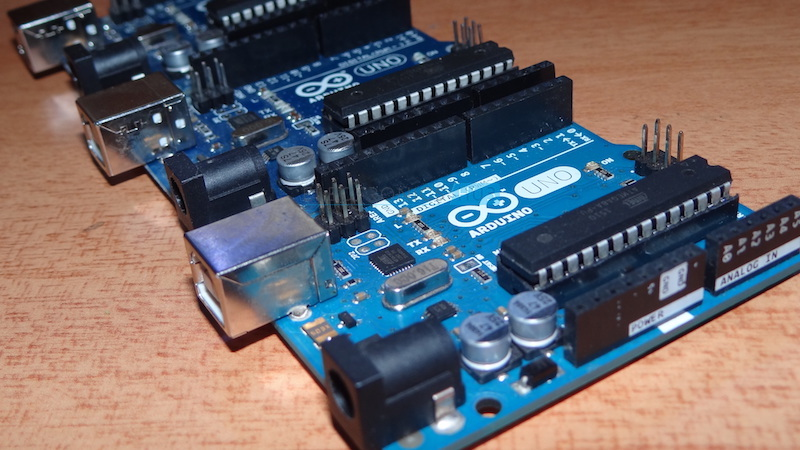
\includegraphics[width=10cm]{pictures/1.jpg}\\
    \textit{Figure 1. An Arduino board.}\\
\end{center}
\medskip
\textbf{Arduino programming language (based on Wiring)}: Arduino programming language can be divided in three main parts:
1) Functions: for controlling the Arduino board and performing computations.
2) Variables: Arduino data types and constants.
3) Structure: the elements of Arduino (C++) code.
Wiring: Wiring is an open-source programming framework for microcontrollers.
Wiring allows writing cross-platform software to control devices attached to a wide range of microcontroller boards to create all kinds of creative coding, interactive objects, spaces or physical experiences. The framework is thoughtfully created with designers and artists in mind to encourage a community where beginners through experts from around the world share ideas, knowledge and their collective experience.\bigskip\\
\textbf{Arduino software (IDE) (based on Processing)}: The open-source Arduino Software (IDE) makes it easy to write code and upload it to the board. This software can be used with any Arduino board.
Processing: Processing is a flexible software sketchbook and a language for learning how to code within the context of the visual arts. Since 2001, Processing has promoted software literacy within the visual arts and visual literacy within technology.
\medskip
\begin{center}
    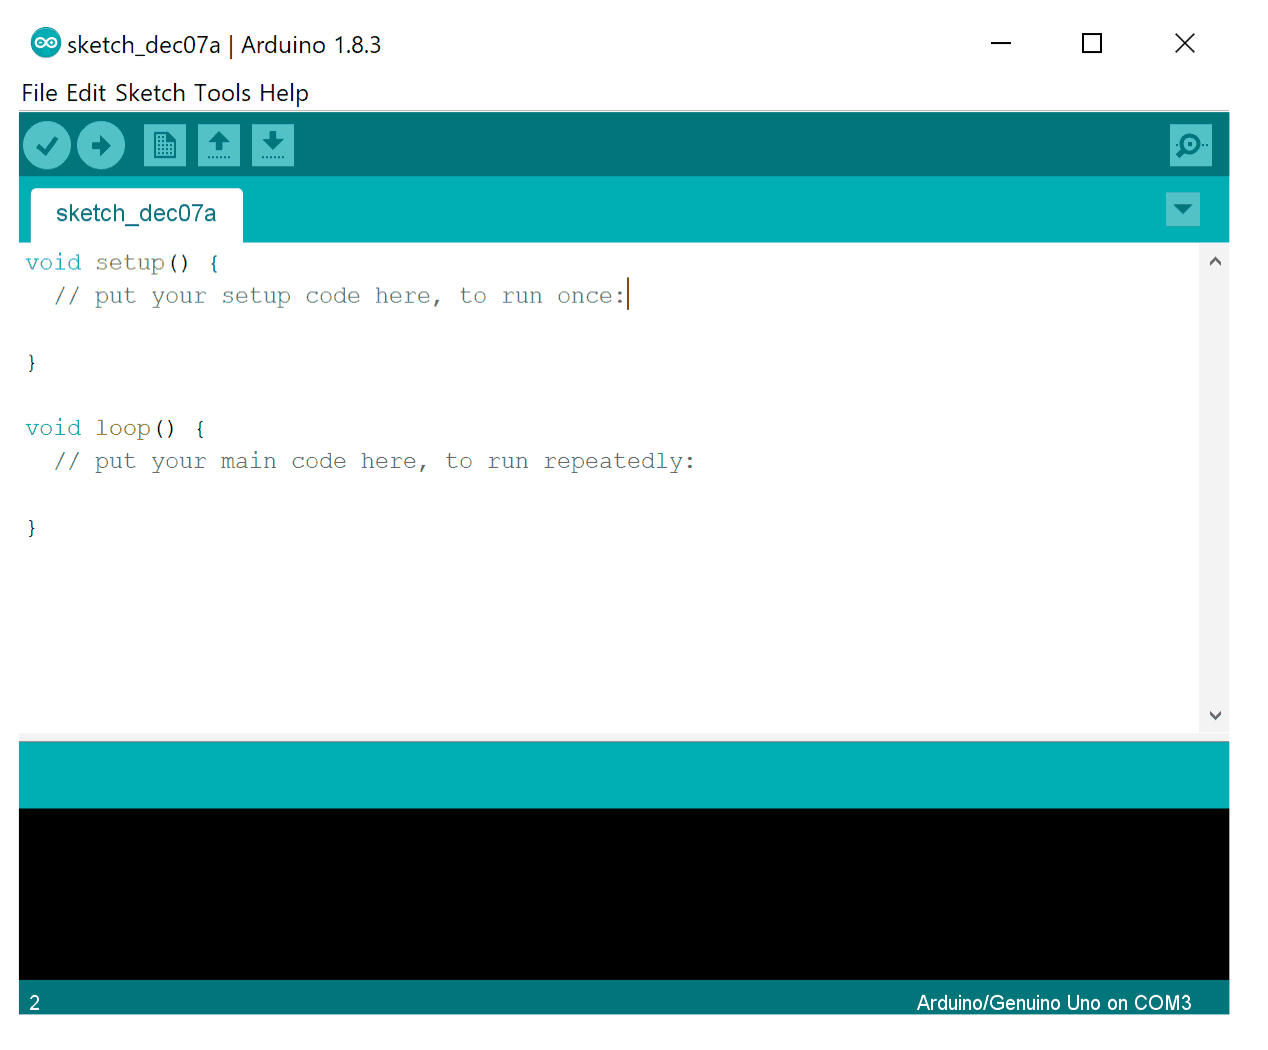
\includegraphics[width=10cm]{pictures/2.png}\\
    \textit{Figure 2. The workplace of Arduino software (IDE).}\\
\end{center}
\medskip
\textbf{Arduino physical boards}: Arduino boards are generally based on microcontrollers from Atmel Corporation like 8, 16 or 32 bit AVR architecture based microcontrollers. The important feature of the Arduino boards is the standard connectors. Using these connectors, we can connect the Arduino board to other devices like LEDs or add-on modules called Shields. There are many types of Arduino boards available in the market: Arduino UNO, Arduino Mega, Arduino Nano, Arduino Micro, Arduino Lilypad, ...
\medskip
\begin{center}
    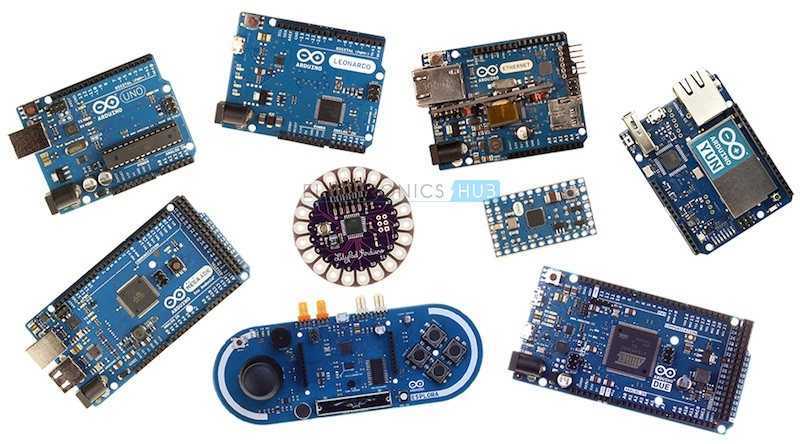
\includegraphics[width=10cm]{pictures/3.jpg}\\
    \textit{Figure 3. Some common types of Arduino boards.}\\
\end{center}
\medskip
\textbf{Advantages of Arduino} over other systems:
\begin{itemize}
    \item Inexpensive - Arduino boards are relatively inexpensive compared to other microcontroller platforms. The least expensive version of the Arduino module can be assembled by hand, and even the pre-assembled Arduino modules cost less than $50$
    \item Cross-platform - The Arduino Software (IDE) runs on Windows, Macintosh OSX, and Linux operating systems. Most microcontroller systems are limited to Windows.
    \item Simple, clear programming environment - The Arduino Software (IDE) is easy-to-use for beginners, yet flexible enough for advanced users to take advantage of as well. For teachers, it's conveniently based on the Processing programming environment, so students learning to program in that environment will be familiar with how the Arduino IDE works.
    \item Open source and extensible software - The Arduino software is published as open source tools, available for extension by experienced programmers. The language can be expanded through C++ libraries, and people wanting to understand the technical details can make the leap from Arduino to the AVR C programming language on which it's based. Similarly, you can add AVR-C code directly into your Arduino programs if you want to.
    \item Open source and extensible hardware - The plans of the Arduino boards are published under a Creative Commons license, so experienced circuit designers can make their own version of the module, extending it and improving it. Even relatively inexperienced users can build the breadboard version of the module in order to understand how it works and save money.
\end{itemize}
\subsubsection{Arduino Uno}
Arduino Uno is a very valuable addition in electronics that consists of a USB interface, 14 digital I/O pins (of which 6 Pins are used for PWM), 6 analog pins and an Atmega328 microcontroller. It also supports 3 communication protocols named Serial, I2C and SPI protocol. In this project, we are going to use the \textbf{Arduino Uno}. A few main features of Arduino Uno are shown in the below figure:
\medskip
\begin{center}
    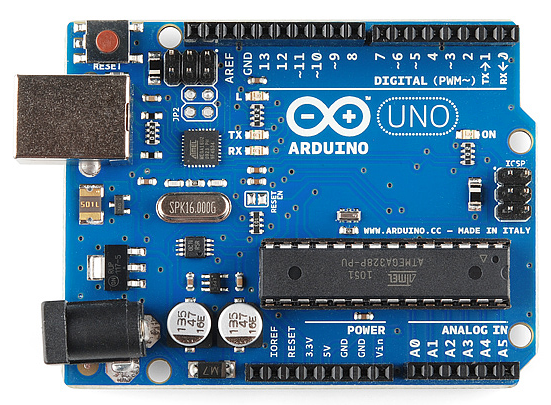
\includegraphics[width=10cm]{pictures/4.png}\\
    \textit{Figure 4. An Arduino Uno board.}\\
\end{center}
\medskip
\begin{center}
    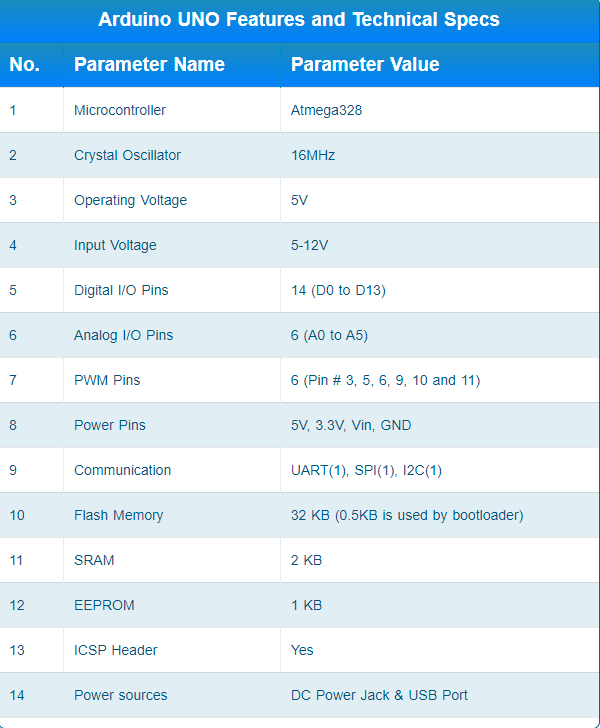
\includegraphics[width=10cm]{pictures/5.png}\\
    \textit{Figure 5. The technical specifications of Arduino Uno.}\\
\end{center}
\medskip

%%%%%%%%%%%%%%%%%%%%%%%%%%%%%%%%%%%%%%%%%%%%%%%%
\subsection{Proteus}
\textbf{Proteus Design Suite} (designed by Labcenter Electronics Ltd.) is a software tool set, mainly used for creating schematics, simulating Electronics and Embedded Circuits and designing PCB Layouts.\bigskip\\
There are 2 main parts of Proteus: Proteus ISIS and Proteus ARES. Proteus ISIS is used by Engineering students and professionals to create schematics and simulations of different electronic circuits. Proteus ARES is used for designing PCB Layouts of electronic circuits. It also provides features related to the three-dimensional view of design in PCB.
\medskip
\begin{center}
    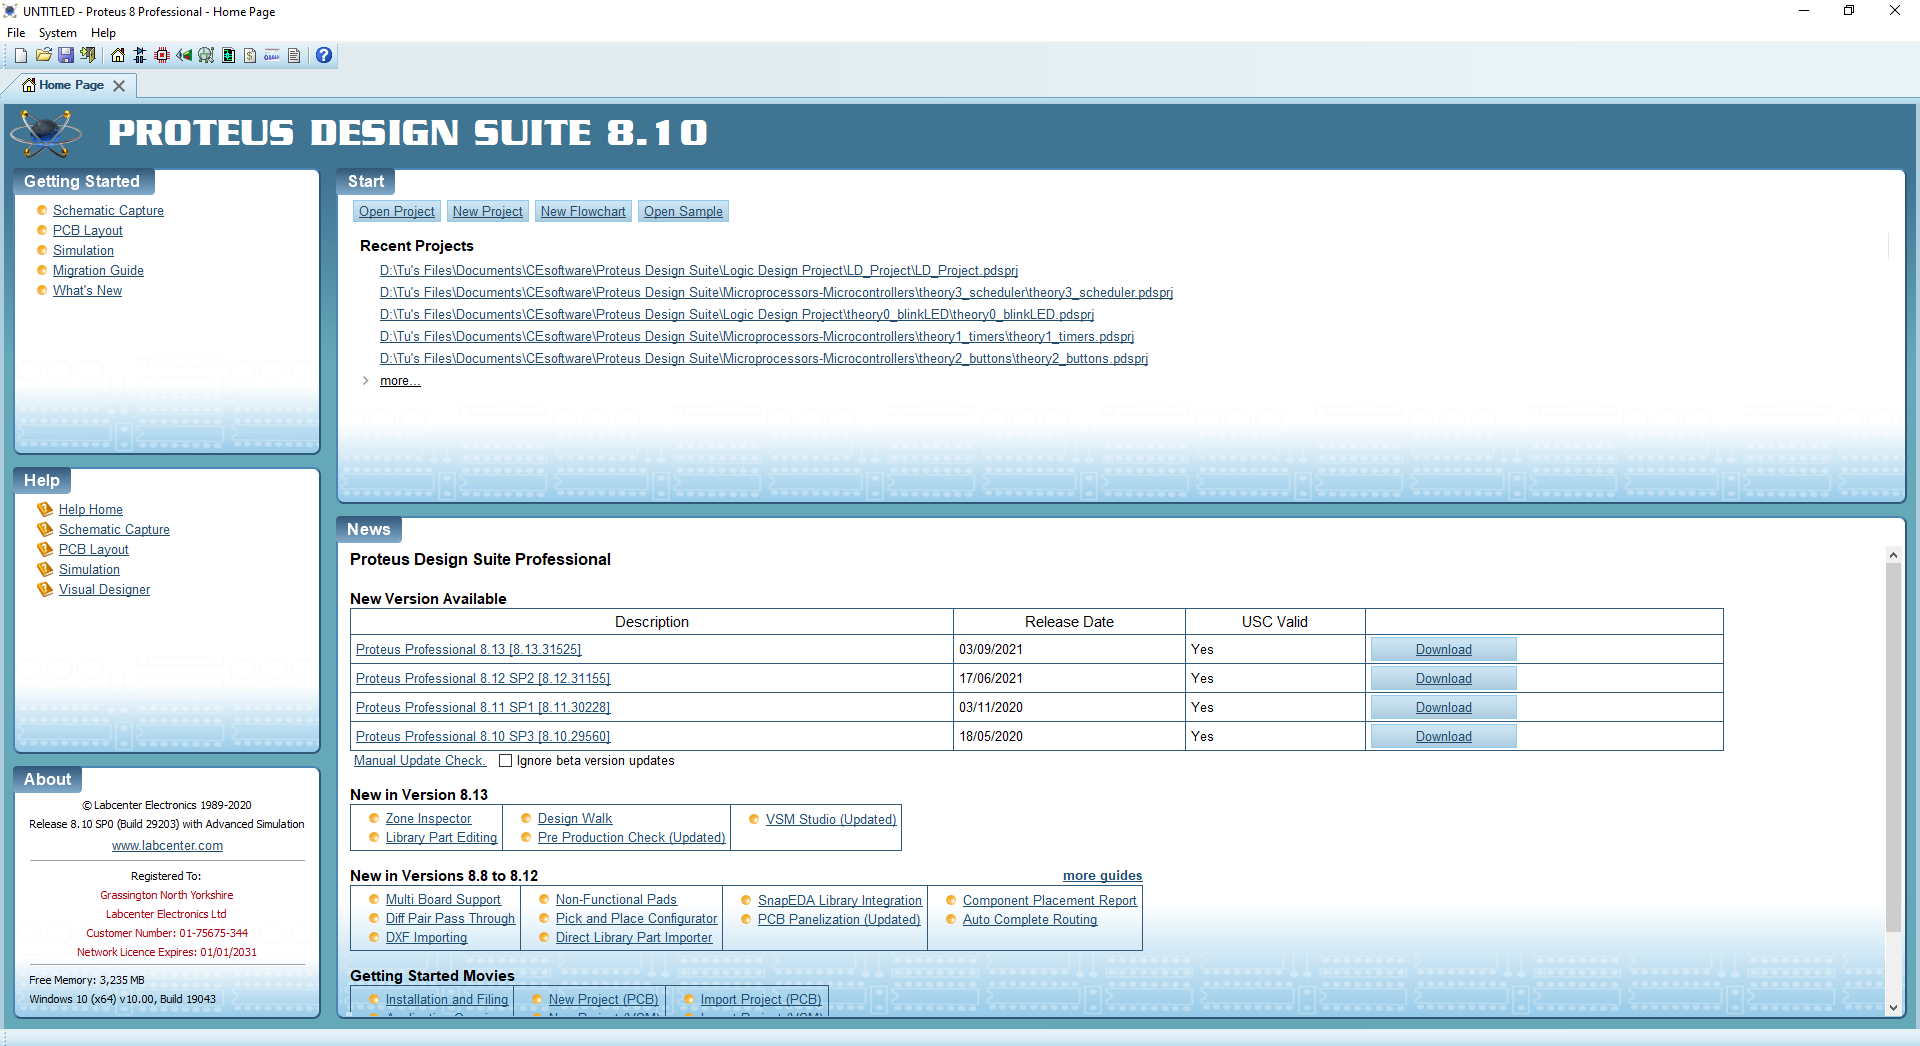
\includegraphics[width=10cm]{pictures/6.png}\\
    \textit{Figure 6. First look of Proteus Design Suite.}\\
\end{center}
\medskip
\textbf{Benefits of using Proteus:}
\begin{itemize}
    \item Designing of circuits on the proteus takes less time than practical construction of the circuit.
    \item The possibility of error is less in software simulation such as loose connection that takes a lot of time to find out connections problems in a practical circuit.
    \item Circuit simulations provide the main feature that some components of circuits are not practical then you can construct your circuit on proteus.
    \item There is zero possibility of burning and damaging of any electronic component in proteus.
    \item The electronic tools that are very expensive can easily get in proteus such as an oscilloscope.
    \item Using proteus you can find different parents of circuits such as current, a voltage value of any component and resistance at any instant which is very difficult in a practical circuit.
\end{itemize}
\medskip

%%%%%%%%%%%%%%%%%%%%%%%%%%%%%%%%%%%%%%%%%%%%%%%%
\subsection{Libraries}
The Arduino environment can be extended through the use of libraries, just like most programming platforms. \textbf{Arduino libraries} are files written in C or C++ (.c, .cpp) which provide your sketches with extra functionality (e.g. the ability to control an LED matrix, or read an encoder, etc.). They were introduced in Arduino 0004. There are three general types of Arduino Libraries: standard libraries, library manager libraries and user installed libraries.\bigskip\\
Some of the most popular libraries include: \textbf{Servo, Firmata, Software Serial, EEPROM, SD, GSM} and \textbf{LiquidCrystal}.\bigskip\\
Let's dig into those two libraries: \textbf{LiquidCrystal.h} and \textbf{DHT.h}\bigskip\\
\textbf{1) LiquidCrystal sensor library}\\
\text{[Description]}: This library allows an Arduino board to control LiquidCrystal displays (\textbf{LCDs}) based on the Hitachi HD44780 (or a compatible) chipset, which is found on most text-based LCDs.\\
\text{[Compatibility]}: This library is compatible with all architectures so you should be able to use it on all the Arduino boards.\\
\text{[NOTE]}: The library works with in either 4- or 8-bit mode (i.e. using 4 or 8 data lines in addition to the rs, enable, and, optionally, the rw control lines).\\
\text{[EXAMPLES]}:
\begin{itemize}
    \item Autoscroll: Shift text right and left.
    \item Blink: Control of the block-style cursor.
    \item Cursor: Control of the underscore-style cursor.
    \item Display: Quickly blank the display without losing what's on it.
    \item Hello World: Displays "hello world!" and the seconds since reset.
    \item Scroll: Scroll text left and right.
    \item Serial Display: Accepts serial input, displays it.
    \item Set Cursor: Set the cursor position.
    \item Text Direction: Control which way text flows from the cursor.
\end{itemize}\bigskip
\textbf{2) DHT sensor library}\\
\text{[Description]}: Arduino library for Temperature and Humidity sensors\\
\text{[Author]}: Adafruit\\
\text{[Maintainer]}: Adafruit\\
\text{[Compatibility]}: This library is compatible with all architectures so you should be able to use it on all the Arduino boards.\\
\text{[NOTE]}: We have two versions of the DHT sensor: DHT11 and DHT22, they look a bit similar and have the same pinout, but have different characteristics. In this project, we are going to use DHT11. Here are the specifications of \textbf{DHT11}:
\begin{itemize}
    \item Ultra low cost
    \item 3 to 5V power and I/O
    \item 2.5mA max current use during conversion (while requesting data)
    \item Good for 20-80$\%$ humidity readings with 5$\%$ accuracy
    \item Good for 0-50°C temperature readings ±2°C accuracy
    \item No more than 1 Hz sampling rate (once every second)
    \item Body size 15.5mm x 12mm x 5.5mm
    \item 4 pins with 0.1" spacing
\end{itemize}
\medskip

%%%%%%%%%%%%%%%%%%%%%%%%%%%%%%%%%%%%%%%%%%%%%%%%
\subsection{First project on Arduino}
\subsubsection{Brief}
\text{[TOPIC]}: BUTTON DEBOUNCING\\
\text{[Description]}: This project aims to toggle an LED using buttons/switches with the issue of debouncing solved.\\
\text{[Board]}: Arduino Uno\\
\text{[Simulation]}: Proteus Design Suite\\
\text{[Timer tick]}: 10 ms\\
\text{[Theory]}: In practice, all mechanical switch contacts bounce (that is, turn on and off, repeatedly, for short period of time) after the switch is closed or opened as shown in the figure below.
\medskip
\begin{center}
    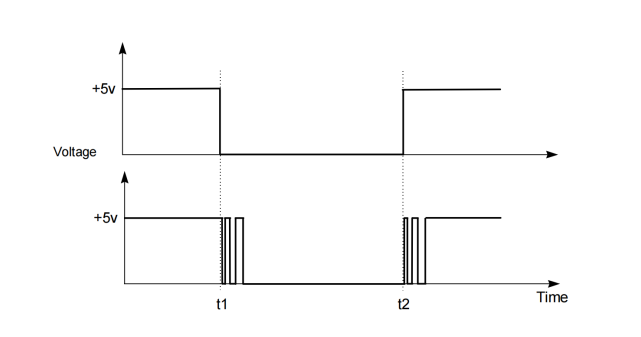
\includegraphics[width=12cm]{pictures/11.png}\\
    \textit{Figure 7.}\\
\end{center}
\medskip
Every system that uses any kind of mechanical switch must deal with the issue of debouncing. The key task is to make sure that one mechanical switch or button action is only read as one action by the MCU, even though the MCU will typically be fast enough to detect the unwanted switch bounces and treat them as separate events. Bouncing can be eliminated by special ICs or by RC circuitry, but in most cases debouncing is done in software because software is “free".\medskip\\
The relevant times we need to consider:
\begin{itemize}
    \item Bounce time: most buttons seem to stop bouncing within 10ms.
    \item Button press time: the shortest time a user can press and release a button seems to be between 50 and 100ms.
    \item Response time: a user notices if the system response is 100ms after the button press, but not if it is 50ms after.
\end{itemize}
Combining all of these times, we can set a few goals
\begin{itemize}
    \item Ignore all bouncing within 10ms
    \item Provide a response within 50ms of detecting a button push (or release)
    \item Be able to detect a 50ms push and a 50ms release
\end{itemize}
\text{[Code explanation]}:
\medskip
\begin{center}
    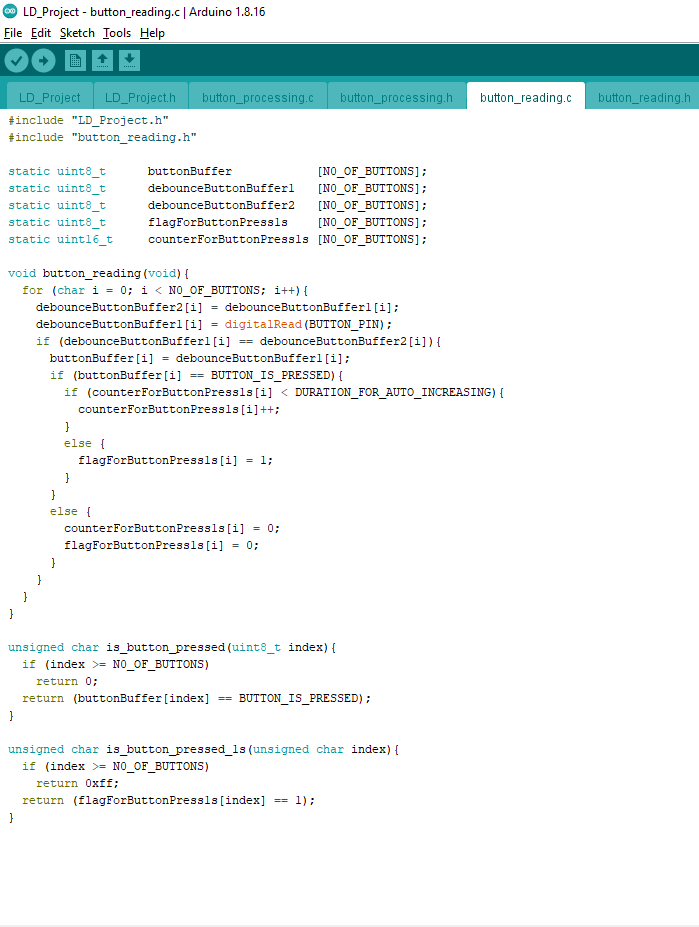
\includegraphics[width=7cm]{pictures/10.png}
    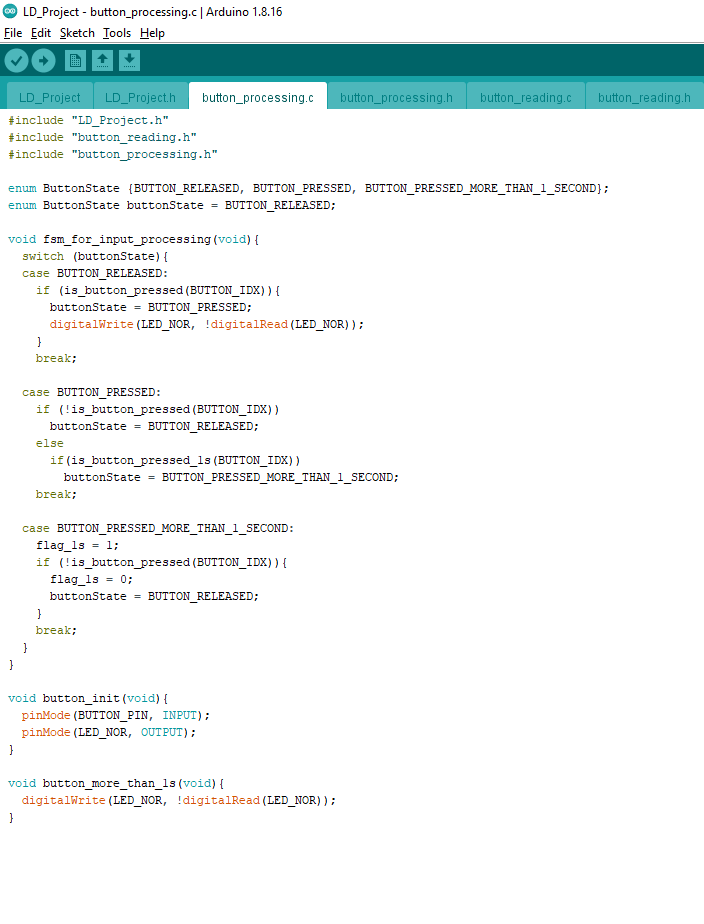
\includegraphics[width=7cm]{pictures/9.png}\\
    \textit{Figure 8.Arduino code of button}\\
\end{center}
\medskip
The debouncing method here is to examine the keys (or buttons or switches) every N milliseconds, where N > 10ms (our specified button bounce upper limit) and N <= 50ms (our specified response time). We then have three possible outcomes every time we read a button:
\begin{itemize}
    \item We read the button in the solid ‘0’ state
    \item We read the button in the solid ‘1’ state
    \item We read the button while it is bouncing (so we will get either a ‘0’ or a ‘1’
\end{itemize}
Note that now we have not two but three button states: active (or pressed), inactive (or released), and indeterminate or invalid (in the middle of filtering, not yet filtered). In most cases we can treat the invalid state the same as the inactive state, since we care in most cases only about when we go active (from whatever state) and when we cease being active (to inactive or invalid). The function button$\_$reading() must be called no more often than our debounce time (10ms).
\subsubsection{System Architecture}
\medskip
\begin{center}
    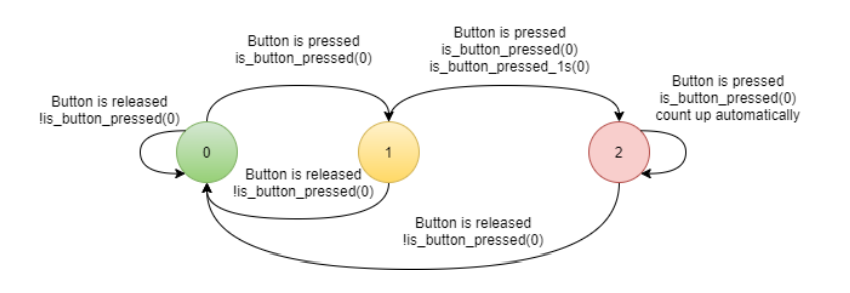
\includegraphics[width=12cm]{pictures/7.png}\\
    \textit{Figure 9.System of button}\\
\end{center}
\medskip
\subsubsection{FSM}
\medskip
\begin{center}
    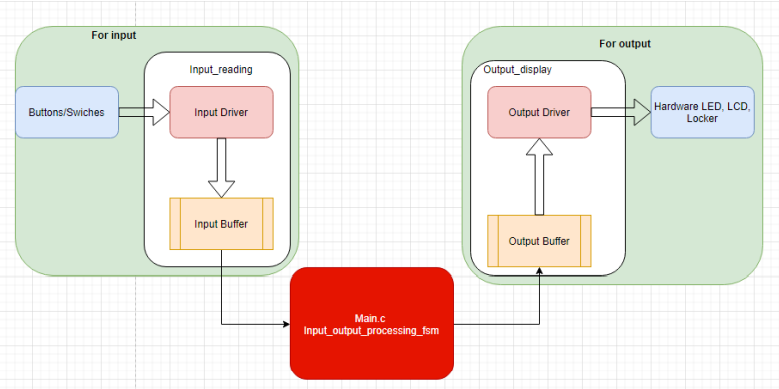
\includegraphics[width=12cm]{pictures/8.png}\\
    \textit{Figure 10.FSM of button}\\
\end{center}
\medskip
\subsubsection{Demo}
\text{[Source]}:\\
\url{https://drive.google.com/file/d/1u8chx10xf5we2SG_iLlJ197xu-ItCKew/view?usp=sharing}

%%%%%%%%%%%%%%%%%%%%%%%%%%%%%%%%%%%%%%%%%%%%%%%%%%%%%%%%%%%%%%%%%%%%%%%%%%%%%%%%%%%%%%%%%%%%%%%%%%%
\newpage
\section{Timer interrupt}
\subsection{Theory}
\textbf{Introduction}\\
Timers are one of the most important features in modern micro-controllers. They allow us to measure how long something takes to execute, create non-blocking code, precisely control pin timing, and even run operating systems.
\medskip
\begin{center}
    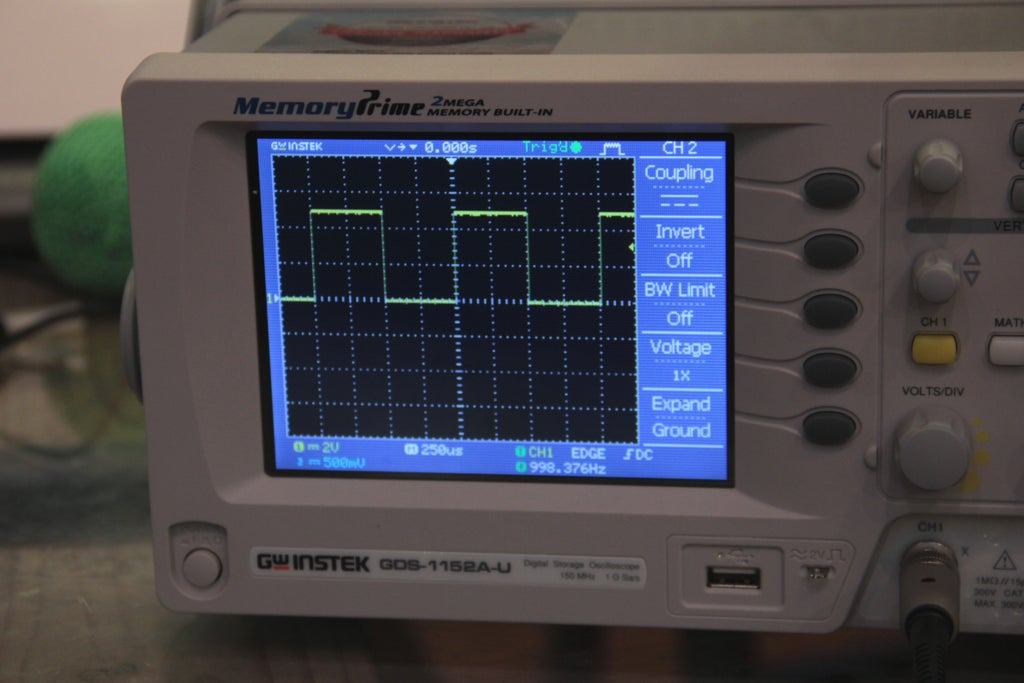
\includegraphics[width=7cm]{pictures/14.jpg}\\
    \textit{Figure 11.}\\
\end{center}
\medskip
\textbf{Arduino Timers}\\
The Arduino Uno has 3 timers:  Timer0, Timer1 and Timer2. Timer interrupts allow you to perform a task at very specifically timed intervals regardless of what else is going on in your code.
\medskip
\begin{center}
    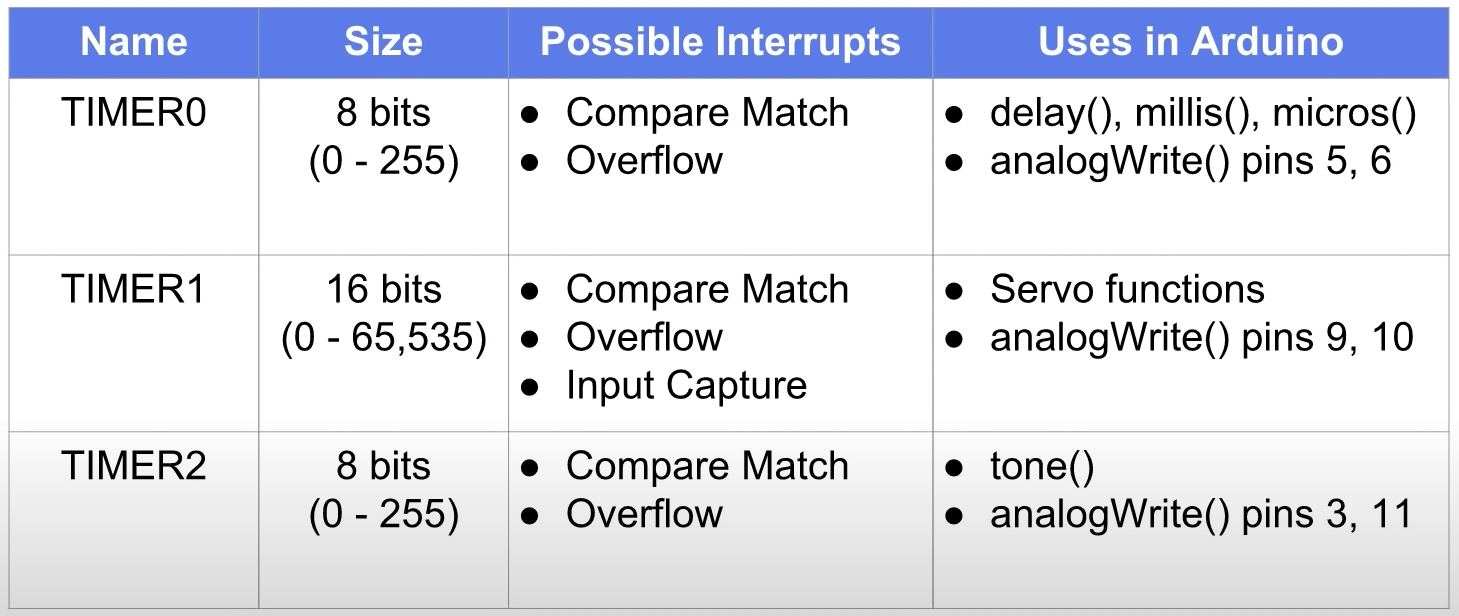
\includegraphics[width=10cm]{pictures/15.png}\\
    \textit{Figure 12. The difference between three timers in Arduino}\\
\end{center}
\medskip
Normally when you write an Arduino sketch the Arduino performs all the commands encapsulated in the loop() {} function in the order that they are written, however, it's difficult to time events in the loop(). Some commands take longer than others to execute, some depend on conditional statements (if, while...) and some Arduino library functions (like digitalWrite or analogRead) are made up of many commands. Arduino timer interrupts allow you to momentarily pause the normal sequence of events taking place in the loop() function at precisely timed intervals, while you execute a separate set of commands. Once these commands are done the Arduino picks up again where it was in the loop().\bigskip\\
\textbf{Interrupts are useful for}:
\begin{itemize}
    \item Measuring an incoming signal at equally spaced intervals (constant sampling frequency)
    \item Calculating the time between two events
    \item Sending out a signal of a specific frequency
    \item Periodically checking for incoming serial data
    \item and much more...
\end{itemize}
\medskip
To do interrupts, for now we will focus on the type called Clear Timer on Compare Match or CTC Mode. The main ideas presented here apply to the Mega and older boards as well, but the setup is a little different and the table below is specific to ATMEL 328/168.\bigskip\\
\textbf{Step 1: Prescalers and the Compare Match Register}
\medskip
\begin{center}
    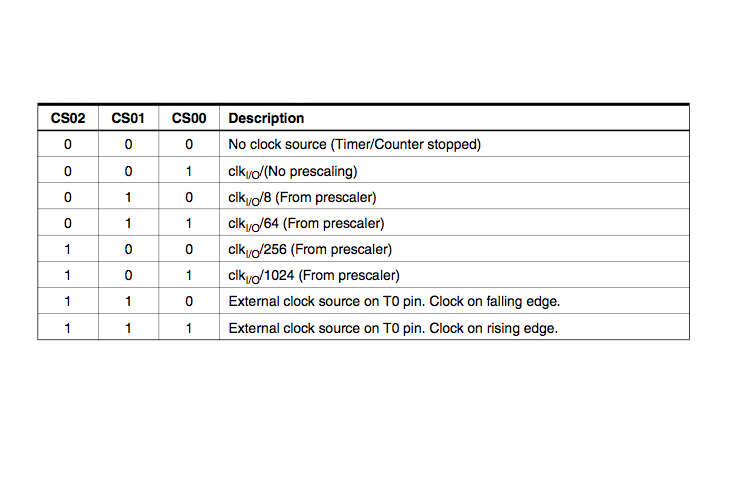
\includegraphics[width=10cm]{pictures/16.png}\\
    \textit{Figure 13.}\\
\end{center}
\medskip
Each of the timers has a counter that is incremented on each tick of the timer's clock. CTC timer interrupts are triggered when the counter reaches a specified value, stored in the compare match register.  Once a timer counter reaches this value it will clear (reset to zero) on the next tick of the timer's clock, then it will continue to count up to the compare match value again.  By choosing the compare match value and setting the speed at which the timer increments the counter, you can control the frequency of timer interrupts.\bigskip\\
The Arduino clock runs at 16MHz, this is the fastest speed that the timers can increment their counters.  At 16MHz each tick of the counter represents 1/16,000,000 of a second (63ns), so a counter will take 10/16,000,000 seconds to reach a value of 9 (counters are 0 indexed), and 100/16,000,000 seconds to reach a value of 99.\bigskip\\
A prescaler dictates the speed of your timer according the the following equation:\bigskip\\
\textbf{(timer speed (Hz)) = (Arduino clock speed (16MHz)) / prescaler}\bigskip\\
Now you can calculate the interrupt frequency with the following equation:\bigskip\\
\textbf{interrupt frequency (Hz) = (Arduino clock speed 16,000,000Hz) / (prescaler * (compare match register + 1))}\\
\textit{(the +1 is in there because the compare match register is zero indexed)}\bigskip\\
Rearranging the equation above, you can solve for the compare match register value that will give your desired interrupt frequency:\bigskip\\
\textbf{compare match register = [ 16,000,000Hz/ (prescaler * desired interrupt frequency) ] - 1}\\
\textit{(remember that when you use timers 0 and 2 this number must be less than 256, and less than 65536 for timer1)}\bigskip\\
\textbf{Step 2: Structuring Timer Interrupts}
\medskip
\begin{center}
    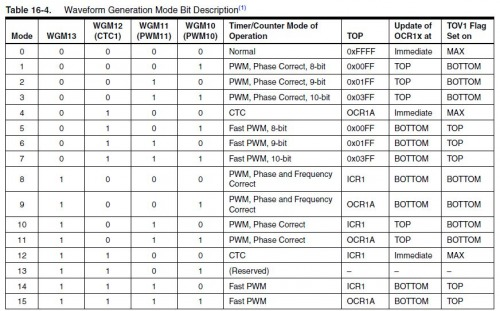
\includegraphics[width=10cm]{pictures/17.jpeg}\\
    \textit{Figure 14.}\\
\end{center}
\medskip
Timer setup code is done inside the setup(){} function in an Arduino sketch.\bigskip\\
The commands you want to execute during these timer interrupts are located in the Arduino sketch encapsulated in the following:\bigskip\\
ISR(TIMER0$\_$COMPA$\_$vect){  //change the 0 to 1 for timer1 and 2 for timer2\\
   //interrupt commands here\\
}\\
This bit of code should be located outside the setup() and loop() functions.  Also, try to keep the interrupt routine as short as possible, especially if you are interrupting at a high frequency.  It may even be worth addressing the ports/pins of the ATMEL chip directly instead of using the digitalWrite() and digitalRead() functions.\bigskip\\
\subsection{Implementation}
\subsubsection{Source code}
\medskip
\begin{center}
    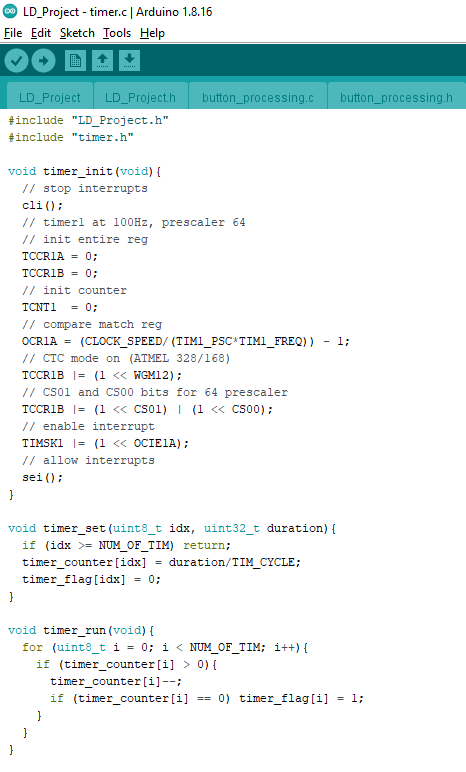
\includegraphics[width=7cm]{pictures/12.png}
    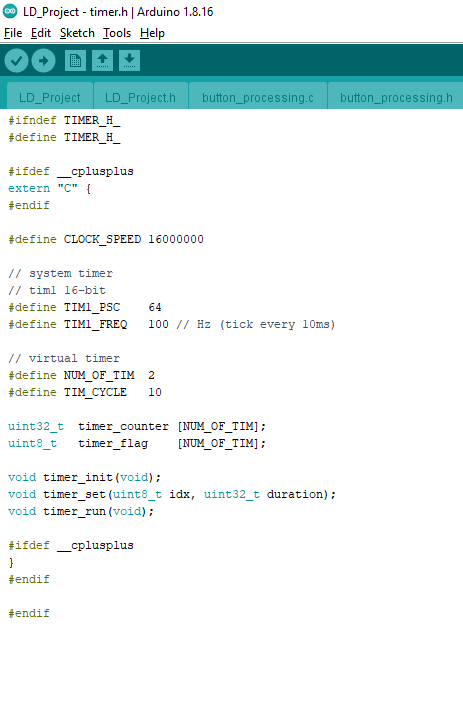
\includegraphics[width=7cm]{pictures/13.png}\\
    \textit{Figure 15.}\\
\end{center}
\medskip

%%%%%%%%%%%%%%%%%%%%%%%%%%%%%%%%%%%%%%%%%%%%%%%%%%%%%%%%%%%%%%%%%%%%%%%%%%%%%%%%%%%%%%%%%%%%%%%%%%%
\newpage
\section{Indoor air monitoring}
\subsection{Theory}
The DHT11 is a basic, ultra low-cost digital temperature and humidity sensor. It uses a capacitive humidity sensor and a thermistor to measure the surrounding air, and spits out a digital signal on the data pin (no analog input pins needed). It is fairly simple to use, but requires careful timing to grab data.\bigskip\\
Since the DHT11 sensor resolution is 1, the values of the humidity and temperature are stored in two variables with type byte (8-bit unsigned).\bigskip\\
The values of the humidity and temperature needs to be displayed on the LCD after the reading, between the DHT11 and the LCD we use the PCF8574.\bigskip\\
The function "lcd.setCursor( , )" in the code highlight below is to set cursor position to index (0,0).
\medskip
\begin{center}
    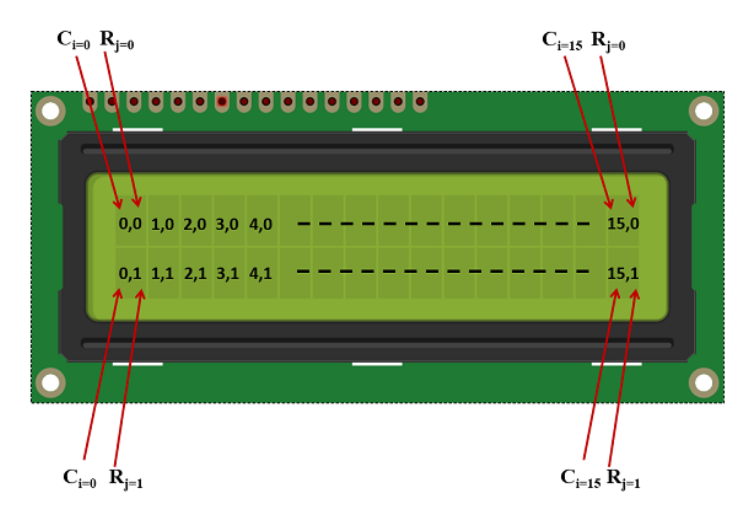
\includegraphics[width=12cm]{pictures/LCD.png}\\
    \textit{Figure 16. LCD}\\
\end{center}
\medskip
\subsection{Implementation}
\subsubsection{Brief}
\text{[TOPIC]}: INDOOR AIR MONITORING\\
\text{[Description]}: This feature aims to receive the data of temperature and humidity from the DHT11 sensor and then display on the LCD.\\
\text{[Board]}: Arduino Uno\\
\text{[Simulation]}: Proteus Design Suite\\
\text{[Timer tick]}: 10 ms\\
\text{[Code highlight]}: 
\medskip
\begin{center}
    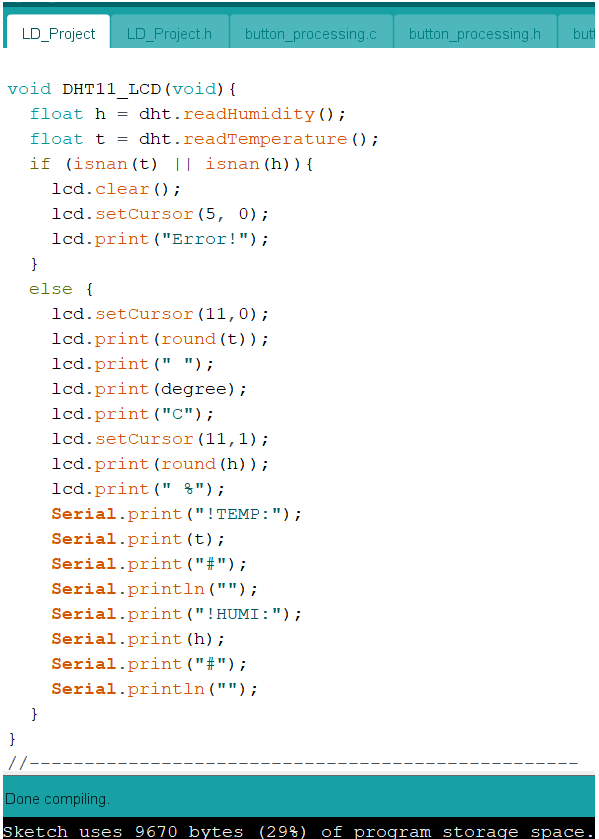
\includegraphics[width=12cm]{pictures/DHT.png}\\
    \textit{Figure 17. void DHT11$\_$LCD()}\\
\end{center}
\subsubsection{System Architecture}
\medskip
\begin{center}
    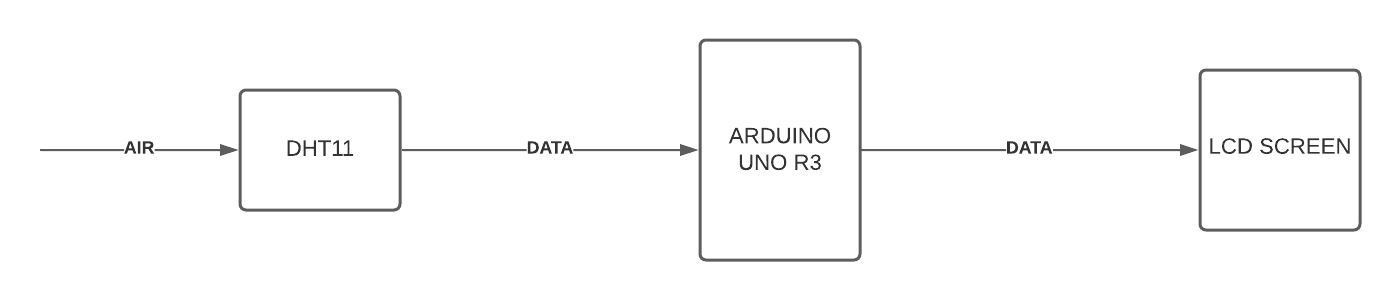
\includegraphics[width=12cm]{pictures/SA_Dht.png}\\
    \textit{Figure 18.System of DHT11}\\
\end{center}
\medskip
\subsubsection{FSM}
\medskip
\begin{center}
    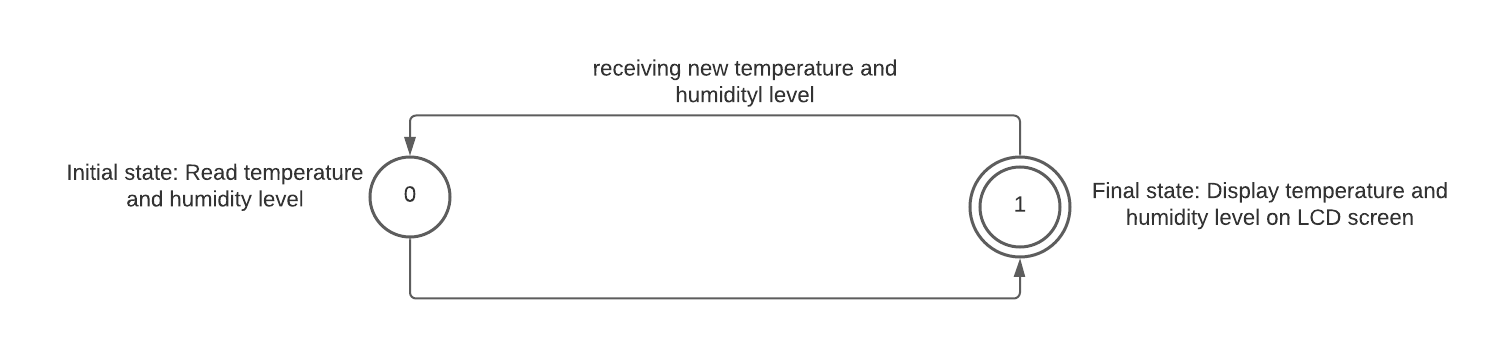
\includegraphics[width=12cm]{pictures/fsm_dht.png}\\
    \textit{Figure 19.FSM of DHT11}\\
\end{center}
\medskip
\subsubsection{Demo}
\text{[Source]}:\\
\url{https://drive.google.com/file/d/1y-he7wXlH7N48s0mZEmDFXeB859PXcwX/view?usp=sharing}

%%%%%%%%%%%%%%%%%%%%%%%%%%%%%%%%%%%%%%%%%%%%%%%%%%%%%%%%%%%%%%%%%%%%%%%%%%%%%%%%%%%%%%%%%%%%%%%%%%%
\newpage
\section{Simple automatic door}
\subsection{Theory}
A passive infrared sensor (PIR sensor) is an electronic sensor that measures infrared (IR) light radiating from objects in its field of view. They are most often used in PIR-based motion detectors. PIR sensors are commonly used in security alarms and automatic lighting applications. PIR sensors detect general movement, but do not give information on who or what moved.\bigskip\\
When an object, such as a person, passes in front of the background, such as a wall, the temperature at that point in the sensor's field of view will rise from room temperature to body temperature, and then back again. The sensor converts the resulting change in the incoming infrared radiation into a change in the output voltage, and this triggers the detection. Objects of similar temperature but different surface characteristics may also have a different infrared emission pattern, and thus moving them with respect to the background may trigger the detector as well.
\subsection{Implementation}
\text{[TOPIC]}: SIMPLE AUTOMATIC DOOR\\
\text{[Description]}: This feature aims to receive the signal of people entering the door (toggled by PIR sensor) to open or close the door automatically.\\
\text{[Board]}: Arduino Uno\\
\text{[Simulation]}: Proteus Design Suite\\
\text{[Timer tick]}: 10 ms\\
\text{[Code highlight]}:
\medskip
\begin{center}
    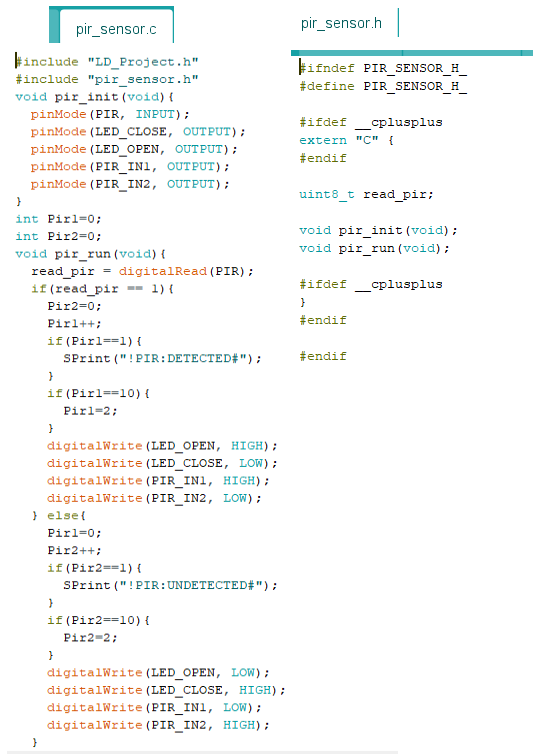
\includegraphics[width=12cm]{pictures/PIR_sensor.png}\\
    \textit{Figure 20.PIR source code}\\
\end{center}
\subsubsection{System Architecture}
\medskip
\begin{center}
    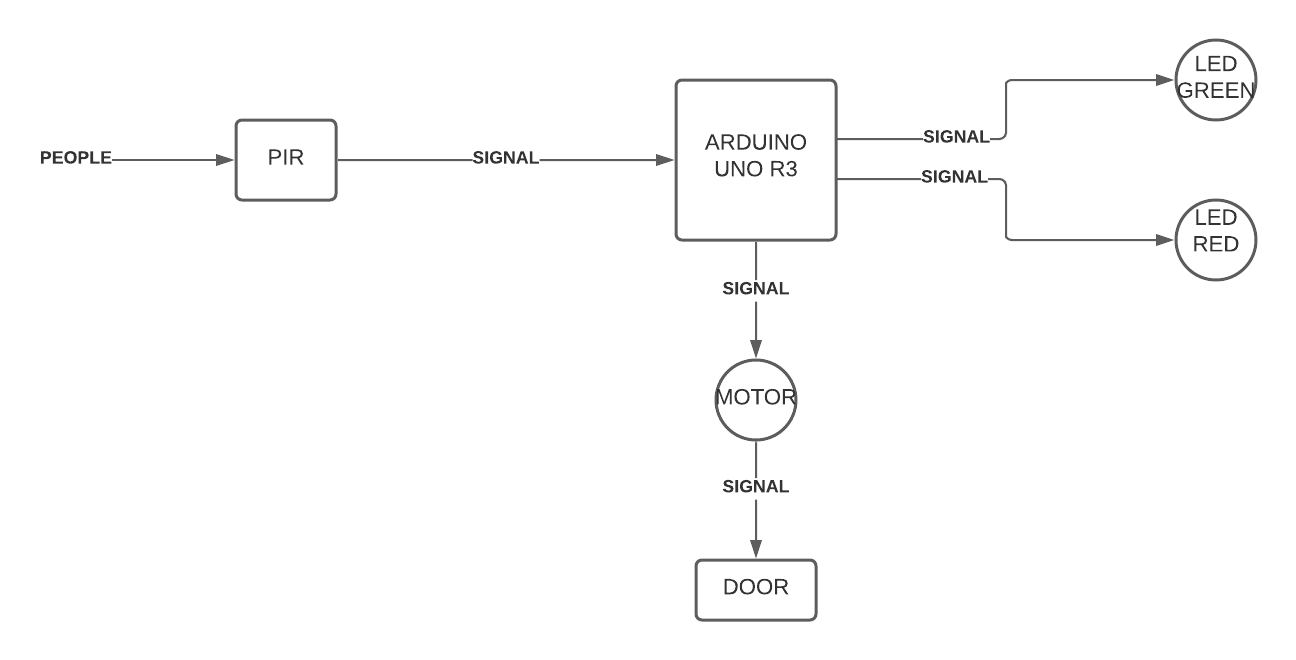
\includegraphics[width=12cm]{pictures/SA_PIR.png}\\
    \textit{Figure 22.FSM of PIR}\\
\end{center}
\medskip
\subsubsection{FSM}
\medskip
\begin{center}
    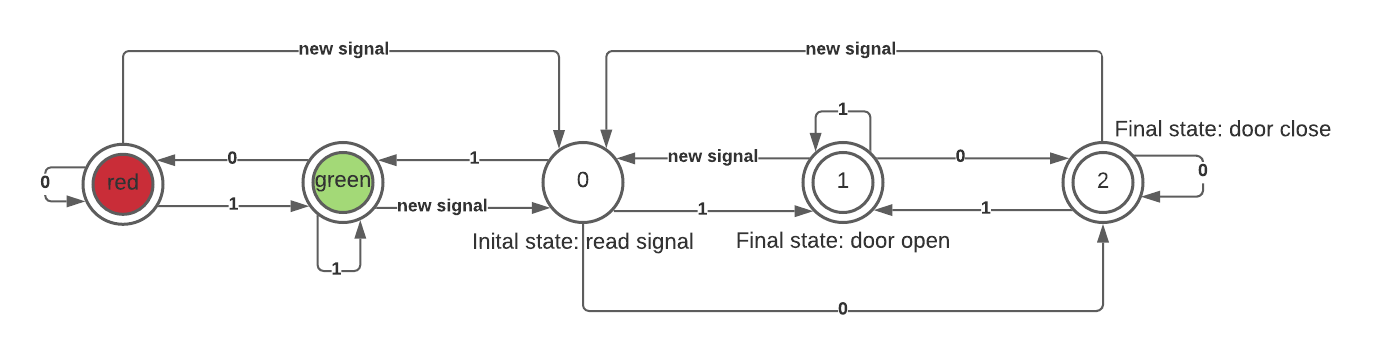
\includegraphics[width=12cm]{pictures/fsm_pir.png}\\
    \textit{Figure 21.System of PIR}\\
\end{center}
\medskip
\subsubsection{Demo}
\text{[Source]}:\\
\url{https://drive.google.com/file/d/19BQTGix81qcRxIpLGfo1kUx_6HuQU1Q6/view?usp=sharing}

%%%%%%%%%%%%%%%%%%%%%%%%%%%%%%%%%%%%%%%%%%%%%%%%%%%%%%%%%%%%%%%%%%%%%%%%%%%%%%%%%%%%%%%%%%%%%%%%%%%
\newpage
\section{Detect soil moisture}
\subsection{Theory}
The Soil Moisture Sensor measures soil moisture grace to the changes in electrical conductivity of the earth (soil resistance increases with drought).\bigskip\\
The electrical resistance is measured between the two electrodes of the sensor.\bigskip\\
A comparator activates a digital output when a adjutable threshold is exceeded.
\subsection{Implementation}
\subsubsection{Brief}
\text{[TOPIC]}: DETECT SOIL MOISTURE\\
\text{[Description]}: This feature aims to read the soil moisture level from the sensor and adjust the pumping motor accordingly.\medskip\\
In details, the soil sensor will be read value between 10s duration, here because we use schematic in Proteus, we will use a "POT-HG" resistor to change the value of the Soil Sensor.Between 10s, The sensor will read the POT-HG resistor and then compare the condition to turn on or off the pumping machine. If the soil moisture is below 70$\%$, we will open the pumping motor, otherwise it will be close.\medskip\\
\text{[Board]}: Arduino Uno\\
\text{[Simulation]}: Proteus Design Suite\\
\text{[Timer tick]}: 10 ms\\
\text{[Code highlight]}:
\medskip
\begin{center}
    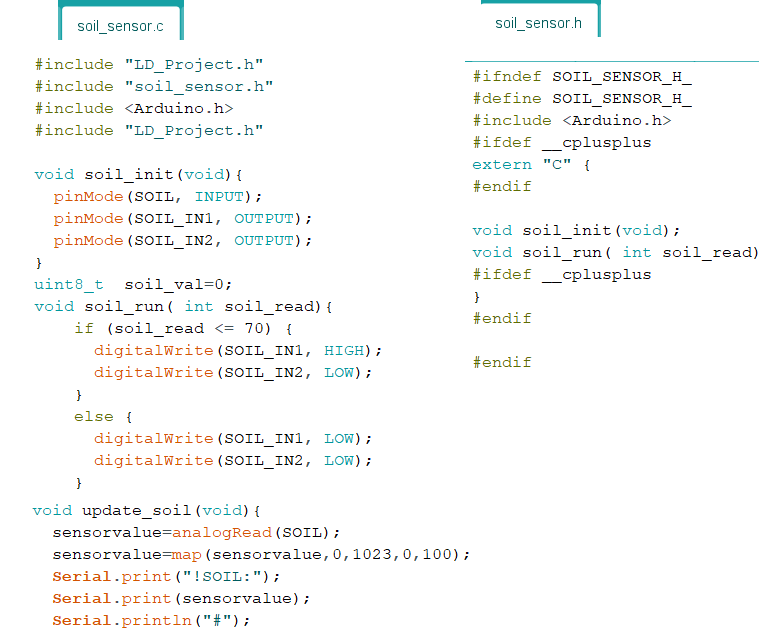
\includegraphics[width=12cm]{pictures/Soil_sensor.png}\\
    \textit{Figure 23.Soil Sensor source code}\\
\end{center}
\subsubsection{System Architecture}
\medskip
\begin{center}
    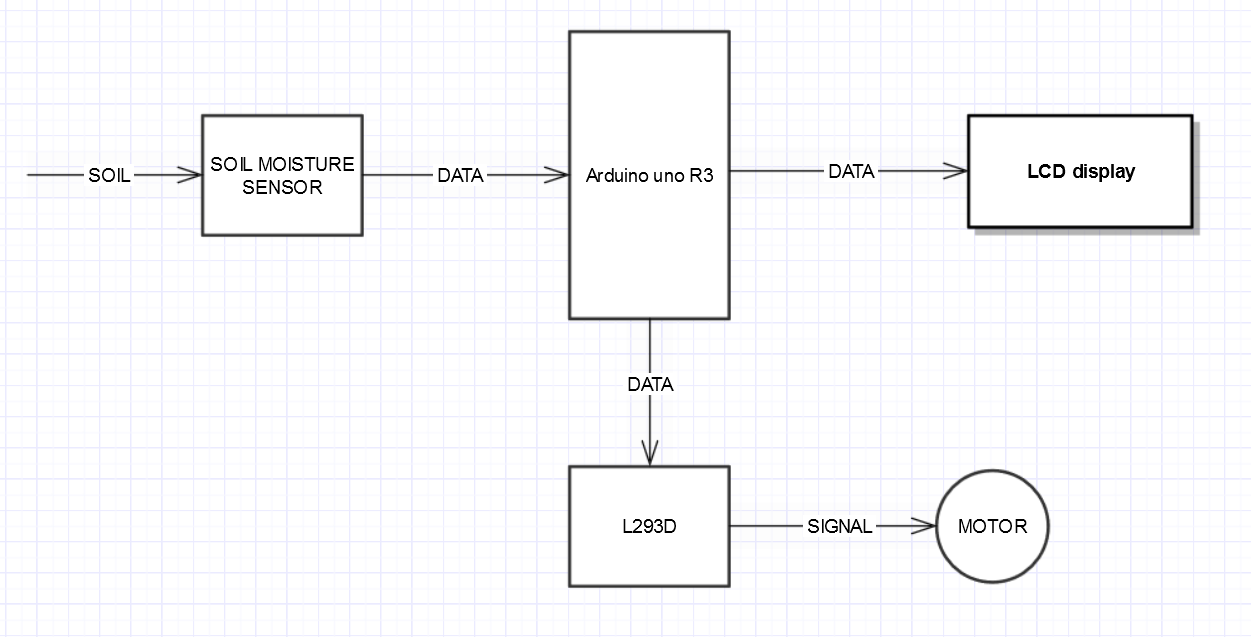
\includegraphics[width=12cm]{pictures/SA_Soil.png}\\
    \textit{Figure 24.System of Soil sensor}\\
\end{center}
\medskip
\subsubsection{FSM}
\medskip
\begin{center}
    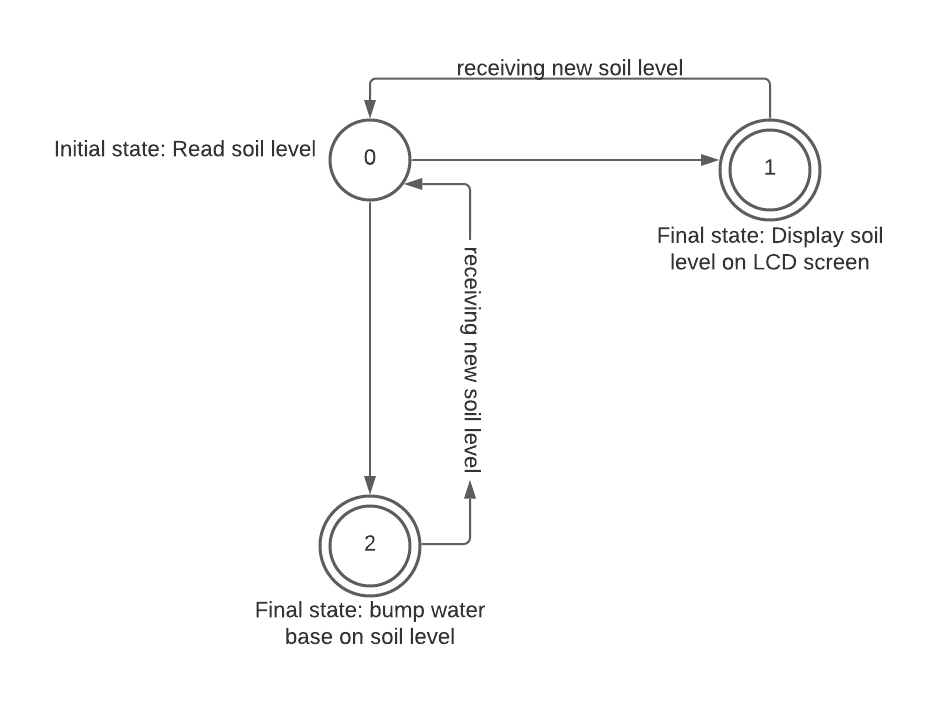
\includegraphics[width=12cm]{pictures/fsm_soil.png}\\
    \textit{Figure 25.FSM soil}\\
\end{center}
\medskip
\subsubsection{Demo}
\text{[Source]}:\\
\url{https://drive.google.com/file/d/1YYLPrjAWYsb3OGAFIwycLhrIA_KLQ5dK/view?usp=sharing}

%%%%%%%%%%%%%%%%%%%%%%%%%%%%%%%%%%%%%%%%%%%%%%%%%%%%%%%%%%%%%%%%%%%%%%%%%%%%%%%%%%%%%%%%%%%%%%%%%%%
\newpage
\section{Detect gas density}
\subsection{Theory}
This gas sensor uses a MQ-2 gas sensor to indicate if there is gas in the area. so the sensor has a threshold value (the threshold value is around the amount of smoke in there is a fire) in that if it goes above it starts alerting people in the vicinity. The alert just shows a red led if the density is high, yellow if medium and green if low or none.\bigskip\\
We use 2 gas sensor, 1 for the checking if the is gas or not, the second one to check the density of the gas.\bigskip\\
Logic:\\
    1. ( Gas sensor=HIGH, Gas Density=HIGH) => Red Led Alert (HIGH)\\
    2. ( Gas sensor=HIGH, Gas Density=LOW) => Yellow Led Alert (MEDIUM)\\
    3. ( Gas sensor=LOW, Gas Density=LOW) => Green Led Alert (LOW)
\subsection{Implementation}
\subsubsection{Brief}
\text{[TOPIC]}: DETECT GAS DENSITY\\
\text{[Description]}: This feature aims to read the density from the sensor and alert us by the three LEDs with three different level of security.\\
\text{[Board]}: Arduino Uno\\
\text{[Simulation]}: Proteus Design Suite\\
\text{[Timer tick]}: 10 ms\\
\text{[Code highlight]}:
\medskip
\begin{center}
    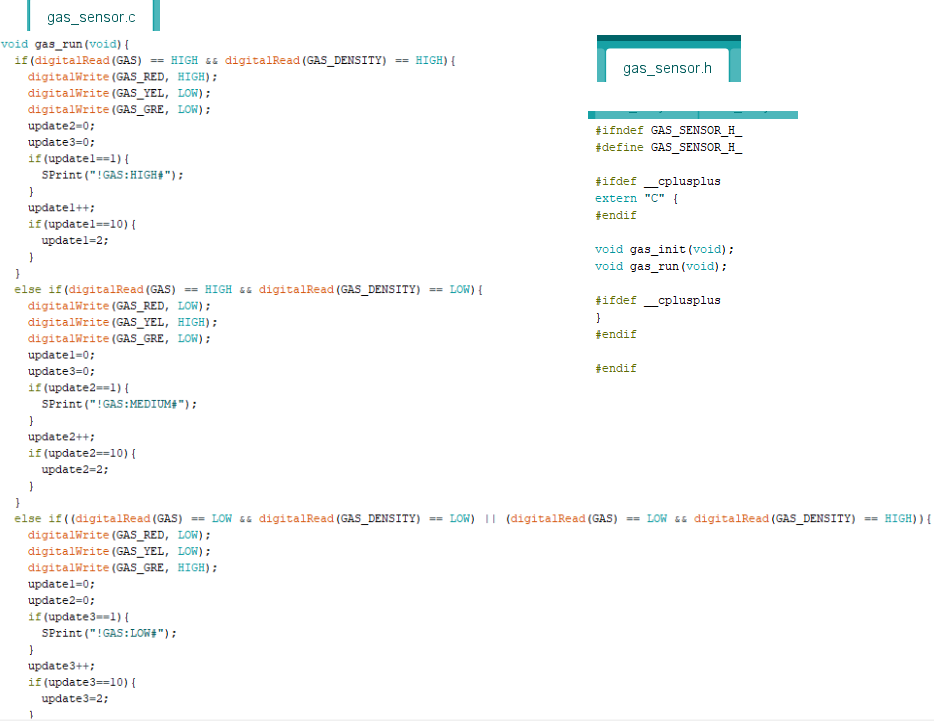
\includegraphics[width=13cm]{pictures/Gas_sensor.png}\\
    \textit{Figure 26.Gas sensor source code}\\
\end{center}
\subsubsection{System Architecture}
\medskip
\begin{center}
    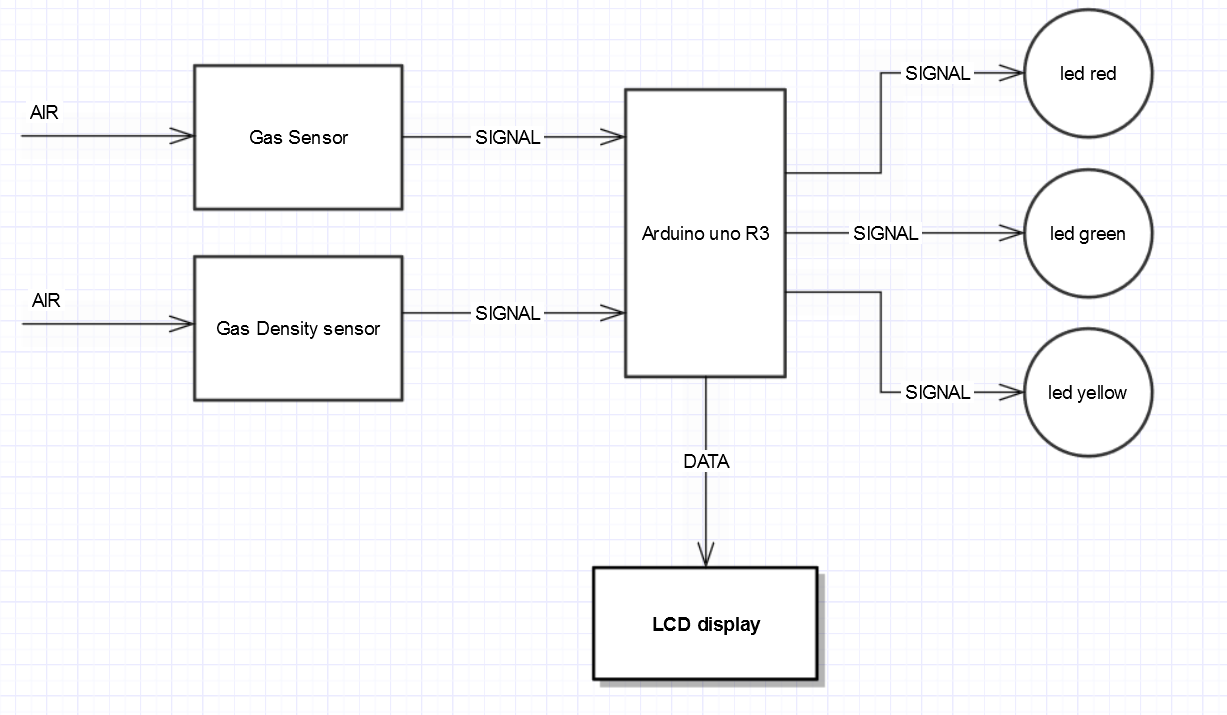
\includegraphics[width=12cm]{pictures/SA_gas.png}\\
    \textit{Figure 27.System of Gas sensor}\\
\end{center}
\medskip
\subsubsection{FSM}
\medskip
\begin{center}
    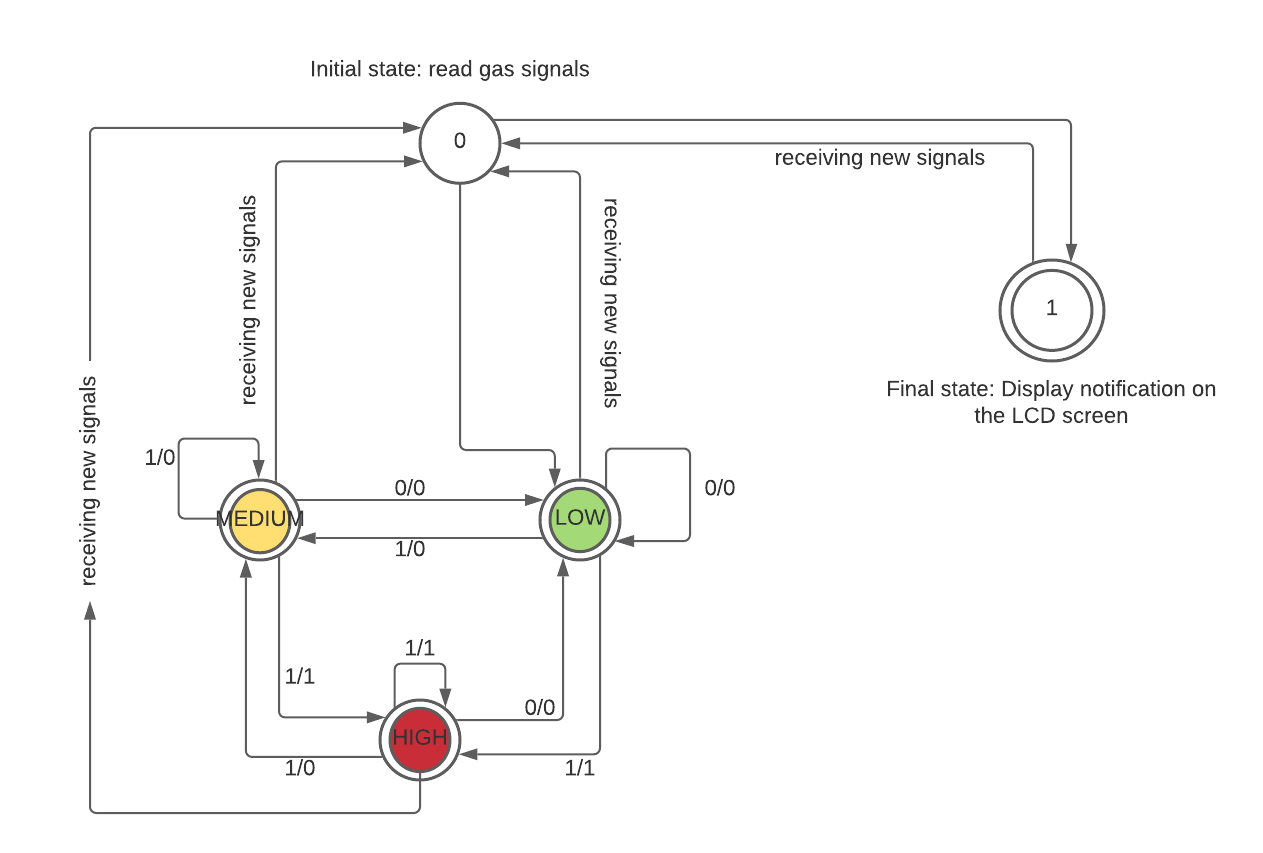
\includegraphics[width=12cm]{pictures/fsm_gas.png}\\
    \textit{Figure 28.FSM of Gas sensor}\\
\end{center}
\medskip
\subsubsection{Demo}
\text{[Source]}:\\
\url{https://drive.google.com/file/d/1XeTtLyJmRPkrlZlS6RKYP_k-cpCXb5to/view?usp=sharing}

%%%%%%%%%%%%%%%%%%%%%%%%%%%%%%%%%%%%%%%%%%%%%%%%%%%%%%%%%%%%%%%%%%%%%%%%%%%%%%%%%%%%%%%%%%%%%%%%%%%
\newpage
\section{Server configuration}
\subsection{Introduction}
This system is Gateway IoT development using Python. This system consists of two main viewing
sections which are an schecmatic on Proteus of the smart home and an Adafruit IO server. The data (such as temperature and humidity)
are displayed on the virtual terminal and Adafruit IO. Connect between block is wireless (Gateway
- Proteus).

\subsubsection{Create virtual ports}
By using the application we can create 2 virtual port. \\
    1. For Gateway (using Python/ Pycharm) (COM5). \\
    2. Connect with COMPIM in Proteus (COM4). \\
\begin{center}
    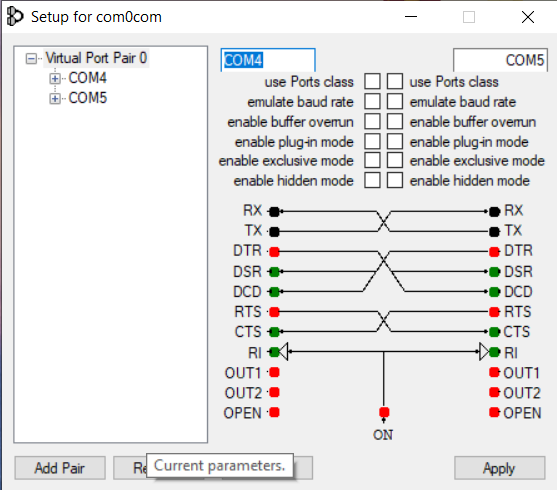
\includegraphics[width=12cm]{pictures/Com0com.png}\\
    \textit{Figure 29.Com0Com}\\
\end{center}
\begin{center}
    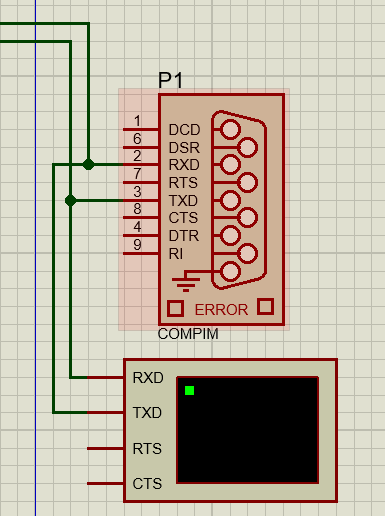
\includegraphics[width=12cm]{pictures/COMPIM.png}\\
    \textit{Figure 30.COMPIM}\\
\end{center}
\begin{center}
    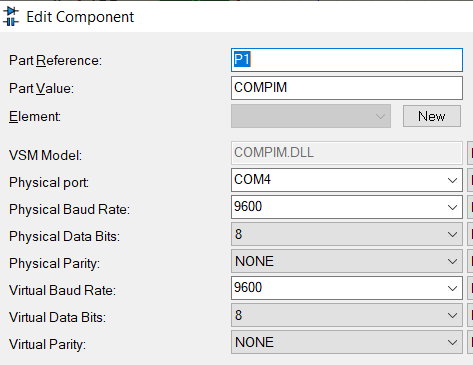
\includegraphics[width=12cm]{pictures/COMPIMsetup.png}\\
    \textit{Figure 31.COMPIM setting}\\
\end{center}
\subsubsection{Create dashboard}
\begin{center}
    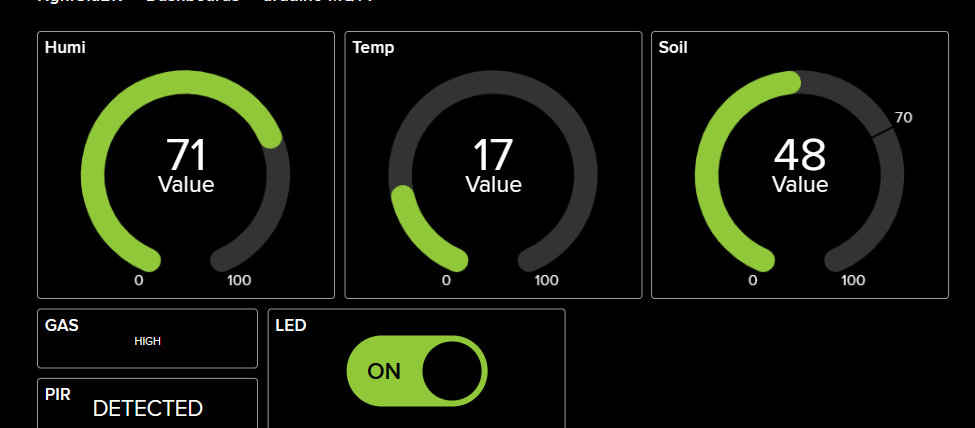
\includegraphics[width=12cm]{pictures/Adafruit.png}\\
    \textit{Figure 32.Adafruit Dashboard}\\
\end{center}
Link for the Ardafruit :"https://io.adafruit.com/NghiGiaBK/dashboards/arduino-mqtt"
%%%%%%%%%%%%%%%%%%%%%%%%%%%%%%%%%%%%%%%%%%%%%%%%%%%%%%%%%%%%%%%%%%%%%%%%%%%%%%%%%%%%%%%%%%%%%%%%%%%
\newpage
\section{Gateway implementation}
\subsection{UART received data}
As the data is received under a format, provide the source code to extract (or decode the data). \\
\begin{center}
    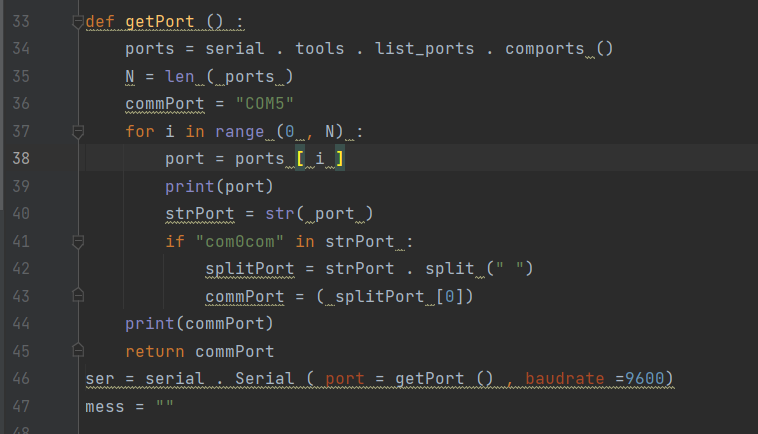
\includegraphics[width=12cm]{pictures/getPort.png}\\
    \textit{Figure 33.Gateway connection}\\
\end{center}
Here we set the gateway will be connected with the Port5 in com0com application which create for us 2 virtual ports, the baudrate will be 9600(as default). \\
\\
The ("ports = serial.tools.listports.comports ()") will be collect all the ports available in the comupter. \\
\begin{center}
    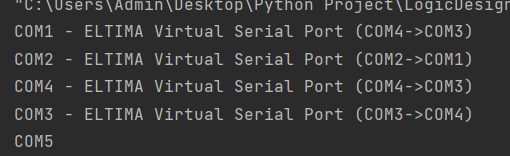
\includegraphics[width=12cm]{pictures/Portavailable.png}\\
    \textit{Figure 34.Ports available}\\
\end{center}
The "for loop" will check for free port so that the gateway can connect with (here we will set it to Com5).\\
\subsection{Data uploading process}
After the sensory data is received by the gateway, the source code to upload the data to MQTT server is presented here. In the case the data is enclosed a format (json string), please present your implemetation for this part.\\
\begin{center}
    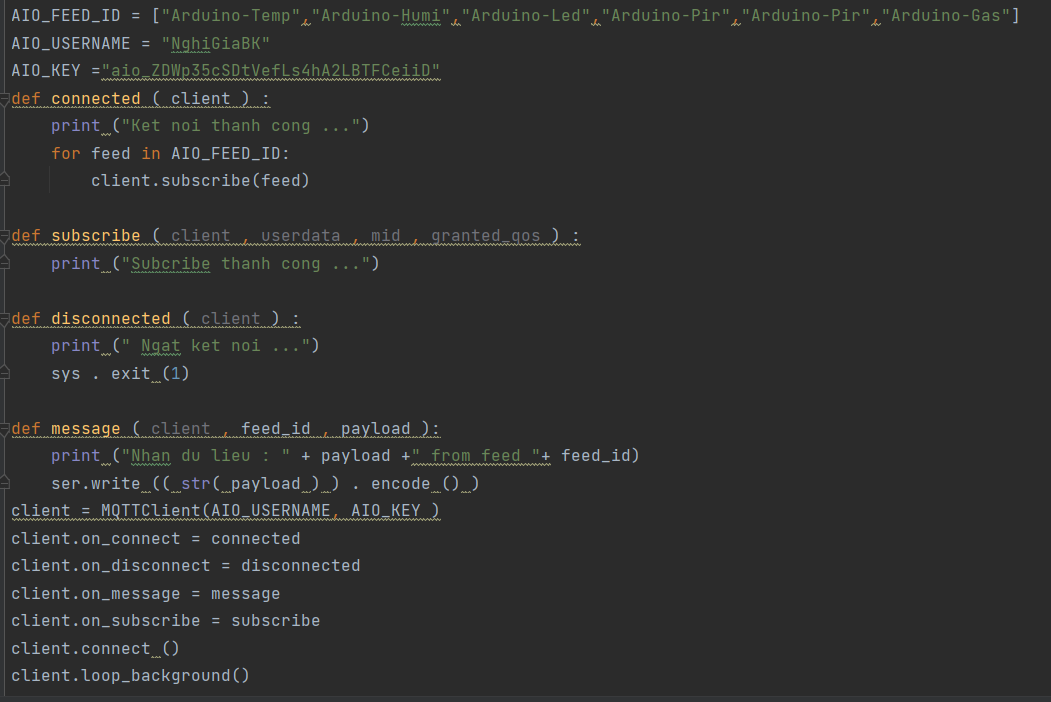
\includegraphics[width=12cm]{pictures/Data_upload1.png}\\
    \textit{Figure 35.}\\
\end{center}
First, if we need to upload some things to Adafruit server we need to create a Adafruit account, then receive AIO-Keys, then in gateway we will subscribe the account which we already create with the funtion ("connected",  and "subscribe")
Second, for each data we need a feed to store those data (like a box), here we have 6 different data so we will create 6 feeds for them. \\
\begin{center}
    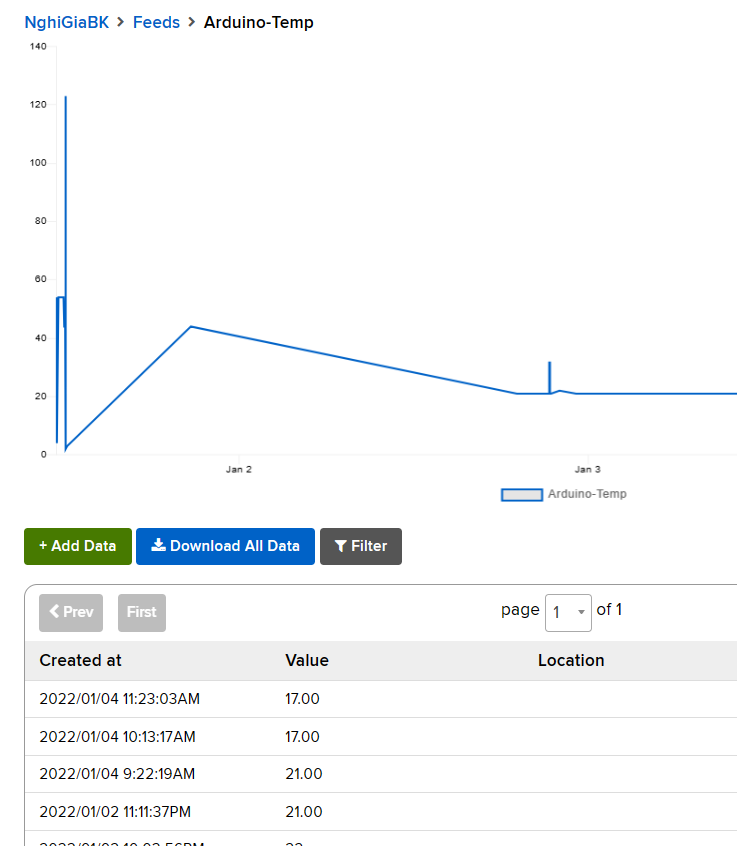
\includegraphics[width=12cm]{pictures/Feeds.png}\\
    \textit{Figure 36.Example of a feed}\\
\end{center}
Then, we need to read the data ( funtion "message") which transfer from the server (feed or dashboard), and then print it to the terminal of python to check and then Serial write to the schematic of Proteus. \\
The ("ser.write ((str(payload)).encode())")  will read the data ( payload) and then send it to the serial connection which we already create.\\ 
\newpage
\subsection{Data received process}
The format of frame data is : !NAME:VALUE \\
\begin{center}
    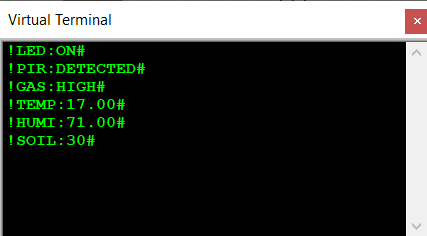
\includegraphics[width=12cm]{pictures/VirtualTerminal.png}\\
    \textit{Figure 37.Virtual Terminal}\\
\end{center}
Because the frame data is following a format, so when we receive a data, we need to split it to the Name and Value, the "Name" will be corresponding to the name of the data and also the feeds, it will publish the value to that feed
\begin{center}
    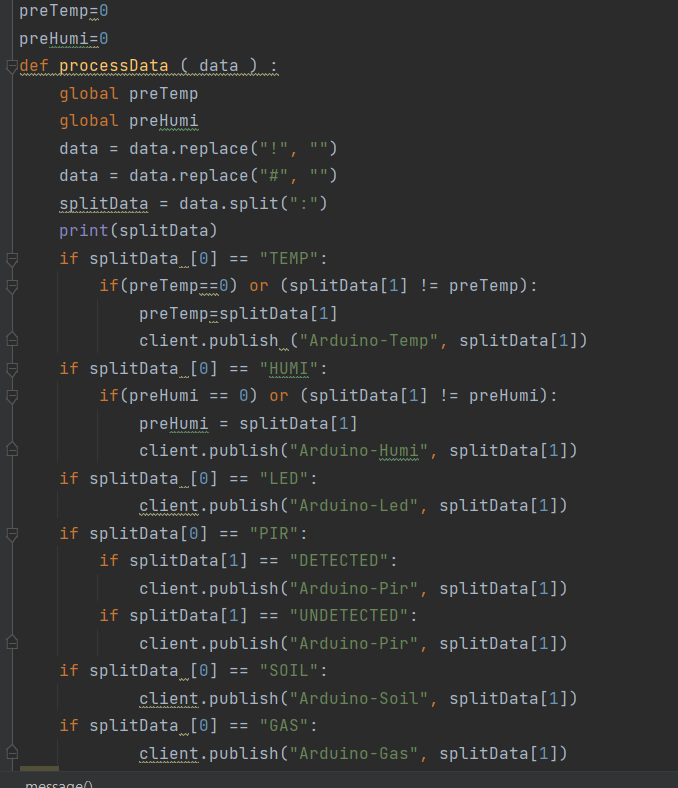
\includegraphics[width=12cm]{pictures/Received_data.png}\\
    \textit{Figure 38.Receive data}\\
\end{center}
\begin{center}
    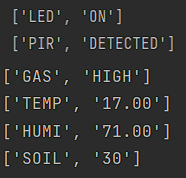
\includegraphics[width=8cm]{pictures/Data_Split.png}\\
    \textit{Figure 39.Data after split}\\
\end{center}
Because the Temp and Humidity will be update every 10 second, if we just upload to the server with the same date, it will overflow server memory and the CPU load, so we will create two integer "preTemp" and "preHumi" to check if the data is different or not between 10s duration.\\
\\
Similarly, in Arduino, if we change some things to get new data, we must create a lock ( just like mutex-lock in OS) to avoid the race condition (other parameters publish data) and it only publish one time until we change new conditions or new values.\\ 
\begin{center}
    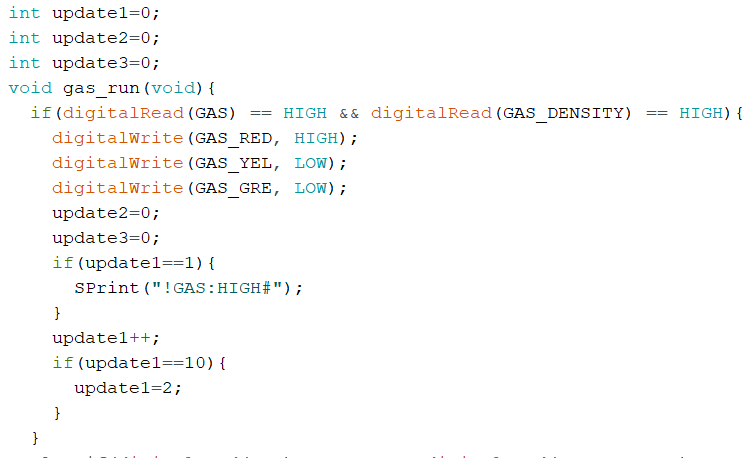
\includegraphics[width=12cm]{pictures/ArduinoSendData.png}\\
    \textit{Figure 40.Avoid race condition in Arduino}\\
\end{center}
%%%%%%%%%%%%%%%%%%%%%%%%%%%%%%%%%%%%%%%%%%%%%%%%%%%%%%%%%%%%%%%%%%%%%%%%%%%%%%%%%%%%%%%%%%%%%%%%%%%
\newpage
\section{Conclusion}
\subsection{Source code}
\url{https://drive.google.com/drive/folders/1mbsSoY6dhdBkLXItWRFM-6DNuYZ6jt6d?usp=sharing}

%%%%%%%%%%%%%%%%%%%%%%%%%%%%%%%%%%%%%%%%%%%%%%%%%%%%%%%%%%%%%%%%%%%%%%%%%%%%%%%%%%%%%%%%%%%%%%%%%%%
\newpage
\addcontentsline{toc}{section}{Reference}

\begin{thebibliography}{80}


\bibitem{bib1}
\url{https://www.arduino.cc/en/}

\bibitem{bib2}
\url{https://www.electronicshub.org/arduino-introduction/}

\bibitem{bib3}
\url{https://learn.sparkfun.com/tutorials/what-is-an-arduino/all}

\bibitem{bib4}
\url{https://www.theengineeringprojects.com/2018/06/introduction-to-arduino-uno.html}

\bibitem{bib5}
\url{https://www.theengineeringprojects.com/2020/01/introduction-to-proteus.html}

\bibitem{bib6}
\url{https://www.theengineeringknowledge.com/introduction-to-proteus/}

\bibitem{bib7}
\url{https://www.arduino.cc/reference/en/libraries/}

\bibitem{bib8}
\url{https://learn.adafruit.com/adafruit-all-about-arduino-libraries-install-use}

\bibitem{bib9}
\url{https://www.youtube.com/watch?v=2kr5A350H7E}

\bibitem{bib10}
\url{https://www.instructables.com/Arduino-Timer-Interrupts/}

\bibitem{bib11}
\url{https://en.wikipedia.org/wiki/Gas_detector}

\bibitem{bib12}
\url{https://en.wikipedia.org/wiki/Soil_moisture_sensor}

\bibitem{bib13}
\url{https://en.wikipedia.org/wiki/Passive_infrared_sensor}

\bibitem{bib14}
\url{https://create.arduino.cc/projecthub/ansh2919/}

\bibitem{bib15}
\url{https://www.theengineeringprojects.com/2013/05/how-to-use-virtual-terminal-in-proteus}

\end{thebibliography}

\end{document}